\documentclass[pdflatex,sn-mathphys-num]{sn-jnl}

\usepackage{mathrsfs}
\usepackage{graphicx}
\usepackage{multirow}
\usepackage{amsmath,amssymb,amsfonts}
\usepackage{amsthm}
\usepackage{mathalpha}
\usepackage[title]{appendix}
\usepackage{xcolor}
\usepackage{textcomp}
\usepackage{manyfoot}
\usepackage{booktabs}
\usepackage{textgreek}
\usepackage[utf8]{inputenc}
\usepackage{algorithm}
\usepackage{algorithmicx}
\usepackage{algpseudocode}
\usepackage{array}
\usepackage{url}
\usepackage{hyperref}

\DeclareUnicodeCharacter{2032}{\ensuremath{\prime}}
\providecommand{\doi}[1]{\href{https://doi.org/#1}{doi:#1}}

% every number quoted in the text is generated from raw results by analysis/make_tables.py
\newcommand{\NumAblFusionSpeedup}{1.13}
\newcommand{\NumAblRqcPasses}{42}
\newcommand{\NumAblRqcPassesNoTiling}{377}
\newcommand{\NumAblSource}{flagship}
\newcommand{\NumAblSwapSpeedup}{16}
\newcommand{\NumAblTilingSpeedup}{2.7}
\newcommand{\NumBuildEightToSixteen}{1.97}
\newcommand{\NumBuildFivetwelveToWide}{0.97}
\newcommand{\NumBuildSixteenMaxN}{28}
\newcommand{\NumBuildSixteenToWide}{1.00}
\newcommand{\NumBuildWideMaxN}{30}
\newcommand{\NumBuildWideToMfour}{1.40}
\newcommand{\NumCpuTriad}{163}
\newcommand{\NumCuScaleOneToEight}{7.7}
\newcommand{\NumEnergyLoopS}{30}
\newcommand{\NumEnergyVsevenRatioMax}{121}
\newcommand{\NumEnergyVsevenRatioMin}{13}
\newcommand{\NumFlagClockMHz}{300}
\newcommand{\NumFlagComputeRoof}{538}
\newcommand{\NumFlagDspPct}{53}
\newcommand{\NumFlagDtwohGhzThirty}{1.3}
\newcommand{\NumFlagDtwohQftThirty}{1.4}
\newcommand{\NumFlagDtwohRqcThirty}{1.4}
\newcommand{\NumFlagDtwohVqeThirty}{1.3}
\newcommand{\NumFlagEnergyGhzThirty}{182}
\newcommand{\NumFlagEnergyQftThirty}{1088}
\newcommand{\NumFlagEnergyRqcThirty}{999}
\newcommand{\NumFlagEnergyVqeThirty}{462}
\newcommand{\NumFlagEngineLut}{26.2}
\newcommand{\NumFlagGhzThirtyEtoE}{4.1}
\newcommand{\NumFlagGhzThirtyExch}{1.3}
\newcommand{\NumFlagGhzThirtyKernel}{1.3}
\newcommand{\NumFlagGhzThirtySweepBw}{141}
\newcommand{\NumFlagLutPct}{40}
\newcommand{\NumFlagPostGhzThirty}{0.14}
\newcommand{\NumFlagPostQftThirty}{0.20}
\newcommand{\NumFlagPostRqcThirty}{0.25}
\newcommand{\NumFlagPostVqeThirty}{0.25}
\newcommand{\NumFlagPowerGhzThirty}{43}
\newcommand{\NumFlagPowerMax}{52}
\newcommand{\NumFlagPowerMin}{39}
\newcommand{\NumFlagPowerQftThirty}{44}
\newcommand{\NumFlagPowerRqcThirty}{48}
\newcommand{\NumFlagPowerVqeThirty}{52}
\newcommand{\NumFlagQftThirtyEtoE}{24.5}
\newcommand{\NumFlagQftThirtyExch}{7.0}
\newcommand{\NumFlagQftThirtyKernel}{15.8}
\newcommand{\NumFlagQftThirtySweepBw}{102}
\newcommand{\NumFlagRqcThirtyEtoE}{20.7}
\newcommand{\NumFlagRqcThirtyExch}{5.7}
\newcommand{\NumFlagRqcThirtyKernel}{13.3}
\newcommand{\NumFlagRqcThirtySweepBw}{67}
\newcommand{\NumFlagVqeThirtyEtoE}{9.0}
\newcommand{\NumFlagVqeThirtyExch}{2.6}
\newcommand{\NumFlagVqeThirtyKernel}{4.7}
\newcommand{\NumFlagVqeThirtySweepBw}{80}
\newcommand{\NumGpuAerDoubleMaxN}{30}
\newcommand{\NumGpuAerDoubleTGhzThirty}{8.09}
\newcommand{\NumGpuAerDoubleTQftThirty}{8.04}
\newcommand{\NumGpuAerDoubleTRqcThirty}{7.99}
\newcommand{\NumGpuAerDoubleTVqeThirty}{7.99}
\newcommand{\NumGpuAerTimeThirtyMax}{4.1}
\newcommand{\NumGpuAerTimeThirtyMin}{4.0}
\newcommand{\NumGpuCudaqDoubleMaxN}{32}
\newcommand{\NumGpuCudaqDoubleTGhzThirty}{8.83}
\newcommand{\NumGpuCudaqDoubleTQftThirty}{9.20}
\newcommand{\NumGpuCudaqSingleMaxN}{33}
\newcommand{\NumGpuCudaqSingleTGhzThirty}{4.30}
\newcommand{\NumGpuCudaqSingleTQftThirty}{14.31}
\newcommand{\NumGpuCusvGainGhzThirty}{1.04}
\newcommand{\NumGpuCusvGainQftThirty}{1.10}
\newcommand{\NumGpuEnergyGhzThirty}{469}
\newcommand{\NumGpuEnergyQftThirty}{641}
\newcommand{\NumGpuEnergyRqcThirty}{585}
\newcommand{\NumGpuEnergyVqeThirty}{491}
\newcommand{\NumGpuMaxN}{32}
\newcommand{\NumGpuPowerGhzThirty}{66}
\newcommand{\NumGpuPowerMax}{88}
\newcommand{\NumGpuPowerMin}{66}
\newcommand{\NumGpuPowerQftThirty}{88}
\newcommand{\NumGpuPowerReadingsMin}{71}
\newcommand{\NumGpuPowerRqcThirty}{81}
\newcommand{\NumGpuPowerVqeThirty}{67}
\newcommand{\NumHbmCeilingPct}{87}
\newcommand{\NumHbmCongestion}{7}
\newcommand{\NumHbmFirstBramPct}{121.5}
\newcommand{\NumHbmPortConnections}{33}
\newcommand{\NumHbmSixteenCopy}{201}
\newcommand{\NumHbmSixteenPerCUCopy}{12.6}
\newcommand{\NumHbmSixteenPerCURead}{12.8}
\newcommand{\NumHbmSixteenPerCUWrite}{12.8}
\newcommand{\NumHbmSixteenRead}{203}
\newcommand{\NumHbmSixteenWrite}{202}
\newcommand{\NumHbmThirtytwoCopy}{399}
\newcommand{\NumHbmThirtytwoPerCUCopy}{12.6}
\newcommand{\NumHbmThirtytwoPerCURead}{9.4}
\newcommand{\NumHbmThirtytwoPerCUWrite}{9.0}
\newcommand{\NumHbmThirtytwoRead}{294}
\newcommand{\NumHbmThirtytwoWrite}{281}
\newcommand{\NumHbmVendorOneBank}{12.1}
\newcommand{\NumJitterAerSpreadMax}{14}
\newcommand{\NumJitterAerSpreadMin}{3}
\newcommand{\NumJitterKAerSpreadMax}{124.9}
\newcommand{\NumJitterKAerSpreadMin}{3.6}
\newcommand{\NumJitterKQulacsSpreadMax}{25.4}
\newcommand{\NumJitterKQulacsSpreadMin}{4.8}
\newcommand{\NumJitterKSvSpreadMax}{12.6}
\newcommand{\NumJitterKSvSpreadMin}{1.3}
\newcommand{\NumJitterKVsevenSpreadMax}{8.9}
\newcommand{\NumJitterKVsevenSpreadMin}{0.4}
\newcommand{\NumJitterQulacsSpreadMax}{27}
\newcommand{\NumJitterQulacsSpreadMin}{4}
\newcommand{\NumJitterSvRqcSixteenPfifty}{32.4}
\newcommand{\NumJitterSvRqcSixteenPnn}{36.9}
\newcommand{\NumJitterSvSpreadMax}{101}
\newcommand{\NumJitterSvSpreadMin}{7}
\newcommand{\NumJitterVsevenSpreadMax}{114}
\newcommand{\NumJitterVsevenSpreadMin}{2}
\newcommand{\NumMaxwFamilies}{4}
\newcommand{\NumMaxwN}{30}
\newcommand{\NumMaxwStateGiB}{8}
\newcommand{\NumMaxwWorstAbs}{5.8\times 10^{-9}}
\newcommand{\NumMaxwWorstInf}{3.7\times 10^{-13}}
\newcommand{\NumMaxwWorstInfThirty}{3.7\times 10^{-13}}
\newcommand{\NumModelEnergyErrMax}{579}
\newcommand{\NumModelEnergyErrMin}{358}
\newcommand{\NumModelPowerErrMax}{58}
\newcommand{\NumModelPowerErrMin}{55}
\newcommand{\NumModelPowerW}{40}
\newcommand{\NumPcieDtoH}{10.9}
\newcommand{\NumPcieHtoD}{10.8}
\newcommand{\NumSpeedupVsevenGhzTwentyEight}{131}
\newcommand{\NumSpeedupVsevenGhzTwentyFour}{72}
\newcommand{\NumSpeedupVsevenMax}{836}
\newcommand{\NumSpeedupVsevenMin}{72}
\newcommand{\NumSpeedupVsevenQftTwentyFour}{836}
\newcommand{\NumSpeedupVsevenRqcTwentyFour}{163}
\newcommand{\NumSpeedupVsevenVqeTwentyFour}{195}
\newcommand{\NumSuiteNewPlatform}{e16w512}
\newcommand{\NumSuitePassNew}{398}
\newcommand{\NumSuitePassVseven}{328}
\newcommand{\NumSuiteThrNew}{10^{-5}}
\newcommand{\NumSuiteThrVseven}{10^{-10}}
\newcommand{\NumSuiteTotal}{398}
\newcommand{\NumSuiteTotalVseven}{396}
\newcommand{\NumSuiteWorstInfNew}{1.6\times10^{-12}}
\newcommand{\NumVsevenBwFracPct}{0.5}
\newcommand{\NumVsevenBwMax}{2.15}
\newcommand{\NumVsevenBwMin}{1.49}
\newcommand{\NumVsevenCyclesPerPair}{10}
\newcommand{\NumVsevenGhzTwentyEightEtoE}{136.1}
\newcommand{\NumVsevenGhzTwentyEightKernel}{122.5}
\newcommand{\NumVsevenKernelFracMin}{73}
\newcommand{\NumVsevenKernelFracMinTwenty}{85}
\newcommand{\NumVsevenOpcodes}{19}
\newcommand{\NumVsevenPowerIdle}{26.8}
\newcommand{\NumVsevenPowerMax}{27.2}
\newcommand{\NumVsevenPowerMin}{26.5}
\newcommand{\NumVsevenUnsupportedTypes}{8}
\newcommand{\NumXmcPeriod}{1.00}
\newcommand{\NumXplatAerRatioGhzThirty}{1.93}
\newcommand{\NumXplatAerRatioQftThirty}{0.75}
\newcommand{\NumXplatAerRatioRqcThirty}{0.84}
\newcommand{\NumXplatAerRatioVqeThirty}{1.15}
\newcommand{\NumXplatBestCpuGhzThirty}{Aer fp64, no fusion}
\newcommand{\NumXplatBestCpuGhzTwentyEight}{Aer fp64, no fusion}
\newcommand{\NumXplatBestCpuGhzTwentyFour}{Qulacs fp64}
\newcommand{\NumXplatBestCpuQftThirty}{Aer fp32}
\newcommand{\NumXplatBestCpuQftTwentyEight}{Aer fp64}
\newcommand{\NumXplatBestCpuQftTwentyFour}{Qulacs fp64}
\newcommand{\NumXplatBestCpuRqcThirty}{Aer fp64}
\newcommand{\NumXplatBestCpuRqcTwentyEight}{qsim fp32}
\newcommand{\NumXplatBestCpuRqcTwentyFour}{qsim fp32}
\newcommand{\NumXplatBestCpuTGhzThirty}{5.0}
\newcommand{\NumXplatBestCpuTGhzTwentyEight}{1.3}
\newcommand{\NumXplatBestCpuTGhzTwentyFour}{0.05}
\newcommand{\NumXplatBestCpuTQftThirty}{18.3}
\newcommand{\NumXplatBestCpuTQftTwentyEight}{4.3}
\newcommand{\NumXplatBestCpuTQftTwentyFour}{0.19}
\newcommand{\NumXplatBestCpuTRqcThirty}{15.7}
\newcommand{\NumXplatBestCpuTRqcTwentyEight}{3.7}
\newcommand{\NumXplatBestCpuTRqcTwentyFour}{0.13}
\newcommand{\NumXplatBestCpuTVqeThirty}{7.5}
\newcommand{\NumXplatBestCpuTVqeTwentyEight}{1.8}
\newcommand{\NumXplatBestCpuTVqeTwentyFour}{0.10}
\newcommand{\NumXplatBestCpuVqeThirty}{Aer fp64}
\newcommand{\NumXplatBestCpuVqeTwentyEight}{Aer fp64}
\newcommand{\NumXplatBestCpuVqeTwentyFour}{qsim fp32}
\newcommand{\NumXplatBestGpuNameGhzThirty}{CUDA-Q fp32}
\newcommand{\NumXplatBestGpuNameQftThirty}{Aer fp32}
\newcommand{\NumXplatBestGpuNameRqcThirty}{Aer fp32}
\newcommand{\NumXplatBestGpuNameVqeThirty}{Aer fp32}
\newcommand{\NumXplatBestGpuRatioGhzThirty}{0.95}
\newcommand{\NumXplatBestGpuRatioQftThirty}{3.36}
\newcommand{\NumXplatBestGpuRatioRqcThirty}{2.86}
\newcommand{\NumXplatBestGpuRatioVqeThirty}{1.23}
\newcommand{\NumXplatBestGpuTGhzThirty}{4.30}
\newcommand{\NumXplatBestGpuTQftThirty}{7.29}
\newcommand{\NumXplatBestGpuTRqcThirty}{7.24}
\newcommand{\NumXplatBestGpuTVqeThirty}{7.28}
\newcommand{\NumXplatCpuFasterOtherThirtyMax}{1.34}
\newcommand{\NumXplatCpuFasterOtherThirtyMin}{1.19}
\newcommand{\NumXplatCpuSmallUs}{54}
\newcommand{\NumXplatFpgaBeatsBestGpu}{GHZ}
\newcommand{\NumXplatFpgaSmallMs}{3.3}
\newcommand{\NumXplatGhzCrossN}{26}
\newcommand{\NumXplatGpuCols}{3}
\newcommand{\NumXplatGpuOverCpuThirtyMax}{2.5}
\newcommand{\NumXplatGpuOverCpuThirtyMin}{0.7}
\newcommand{\NumXplatGpuRatioGhzThirty}{0.57}
\newcommand{\NumXplatGpuRatioGhzTwentyEight}{0.56}
\newcommand{\NumXplatGpuRatioGhzTwentyFour}{0.55}
\newcommand{\NumXplatGpuRatioQftThirty}{3.36}
\newcommand{\NumXplatGpuRatioQftTwentyEight}{2.79}
\newcommand{\NumXplatGpuRatioQftTwentyFour}{1.92}
\newcommand{\NumXplatGpuRatioRqcThirty}{2.86}
\newcommand{\NumXplatGpuRatioRqcTwentyEight}{2.59}
\newcommand{\NumXplatGpuRatioRqcTwentyFour}{1.61}
\newcommand{\NumXplatGpuRatioThirtyMax}{3.36}
\newcommand{\NumXplatGpuRatioThirtyMin}{0.57}
\newcommand{\NumXplatGpuRatioVqeThirty}{1.23}
\newcommand{\NumXplatGpuRatioVqeTwentyEight}{1.19}
\newcommand{\NumXplatGpuRatioVqeTwentyFour}{1.21}
\newcommand{\NumXplatGpuTGhzThirty}{7.16}
\newcommand{\NumXplatGpuTGhzTwentyEight}{1.85}
\newcommand{\NumXplatGpuTGhzTwentyFour}{0.18}
\newcommand{\NumXplatGpuTQftThirty}{7.29}
\newcommand{\NumXplatGpuTQftTwentyEight}{1.93}
\newcommand{\NumXplatGpuTQftTwentyFour}{0.24}
\newcommand{\NumXplatGpuTRqcThirty}{7.24}
\newcommand{\NumXplatGpuTRqcTwentyEight}{1.90}
\newcommand{\NumXplatGpuTRqcTwentyFour}{0.26}
\newcommand{\NumXplatGpuTVqeThirty}{7.28}
\newcommand{\NumXplatGpuTVqeTwentyEight}{1.89}
\newcommand{\NumXplatGpuTVqeTwentyFour}{0.21}
\newcommand{\NumXplatOtherWinsN}{0}
\newcommand{\NumXplatRatioGhzThirty}{1.21}
\newcommand{\NumXplatRatioGhzTwentyEight}{1.21}
\newcommand{\NumXplatRatioGhzTwentyFour}{0.47}
\newcommand{\NumXplatRatioOtherThirtyMax}{0.84}
\newcommand{\NumXplatRatioOtherThirtyMin}{0.75}
\newcommand{\NumXplatRatioQftThirty}{0.75}
\newcommand{\NumXplatRatioQftTwentyEight}{0.80}
\newcommand{\NumXplatRatioQftTwentyFour}{0.41}
\newcommand{\NumXplatRatioRqcThirty}{0.76}
\newcommand{\NumXplatRatioRqcTwentyEight}{0.76}
\newcommand{\NumXplatRatioRqcTwentyFour}{0.31}
\newcommand{\NumXplatRatioThirtyMax}{1.21}
\newcommand{\NumXplatRatioThirtyMin}{0.75}
\newcommand{\NumXplatRatioTwentyFourMax}{0.47}
\newcommand{\NumXplatRatioTwentyFourMin}{0.31}
\newcommand{\NumXplatRatioVqeThirty}{0.84}
\newcommand{\NumXplatRatioVqeTwentyEight}{0.81}
\newcommand{\NumXplatRatioVqeTwentyFour}{0.38}

\theoremstyle{thmstyleone}
\newtheorem{theorem}{Theorem}
\theoremstyle{thmstylethree}
\newtheorem{definition}{Definition}

\raggedbottom

\begin{document}

\title[FPGA Based Quantum Circuit Simulator]{FPGA Based Quantum Circuit Simulator: Processing 30 Qubit Systems}

\author*[1]{\fnm{Abhishek} \sur{Tiwari}}\email{abhishek@cdac.in}
\author*[1]{\fnm{Nasir} \sur{Ali}}\email{nasirali2607@gmail.com}
\author[1]{\fnm{Nadeem} \sur{Khan}}\email{khannadeem73637@gmail.com}
\author[1]{\fnm{Imam} \sur{Mazhar}}\email{imammazhar@cdac.in}
\author[1]{\fnm{Karan} \sur{Islur}}\email{karanislur2003@gmail.com}
\author[1]{\fnm{Himanshu} \sur{Gupta}}\email{himanshugupta@cdac.in}
\author[2]{\fnm{Sachin} \sur{Kumar}}\email{skumar@cic.du.ac.in}
\author[2]{\fnm{Pankaj} \sur{Tyagi}}\email{pankajtyagi@cic.du.ac.in}
\author[3]{\fnm{Rahul} \sur{Kumar Neiwal}}\email{rahul.neiwal@meity.gov.in}

\affil*[1]{\orgdiv{Embedded Systems Division}, \orgname{Centre for Development of Advanced Computing}, \orgaddress{\city{Noida}, \postcode{201307}, \country{India}}}
\affil[2]{\orgdiv{Cluster Innovation Centre}, \orgname{University of Delhi}, \orgaddress{\city{New Delhi}, \postcode{110007}, \country{India}}}
\affil[3]{\orgdiv{Electronics Division}, \orgname{Ministry of Electronics and Information Technology}, \orgaddress{\city{New Delhi}, \postcode{110003}, \country{India}}}

\abstract{Statevector simulation of quantum circuits is limited by memory bandwidth, and data-centre FPGAs with high-bandwidth memory offer bandwidth comparable to workstation GPUs. We present a statevector simulator for the AMD Alveo U55C that executes every gate with one multiplexed $2\times2$ datapath primitive applied to on-chip tiles of the state, runs one streaming engine per HBM pseudo-channel and performs qubit remaps on the card. A single card simulates 30 qubits in single precision. We measure the memory ceilings of the card (\NumHbmThirtytwoCopy~GB/s over 32 pseudo-channels, \NumHbmSixteenPerCURead~GB/s per channel), study engines, channels, port width, tiling, gate fusion and exchange, and verify correctness with a fidelity suite of \NumSuiteTotal{} cases started from entangled states, all of which pass. Compared with an existing HBM kernel for the same card, end-to-end time falls by \NumSpeedupVsevenMin to \NumSpeedupVsevenMax$\times$ at 24 qubits and energy per circuit by \NumEnergyVsevenRatioMin to \NumEnergyVsevenRatioMax$\times$. Against Qiskit Aer, qsim and Qulacs on a 128-core server, the card is faster for bandwidth-bound circuits from \NumXplatGhzCrossN{} qubits (GHZ-30 in \NumFlagGhzThirtyEtoE~s, \NumXplatRatioGhzThirty$\times$ faster than the best CPU configuration), while for compute-bound circuits (QFT, random circuits, VQE ansatz) the server remains faster, needing \NumXplatRatioOtherThirtyMin to \NumXplatRatioOtherThirtyMax{} of the FPGA time at 30 qubits. The card draws \NumFlagPowerMin to \NumFlagPowerMax~W while simulating. An NVIDIA A100 with Qiskit Aer and CUDA-Q is faster than the card for compute-bound circuits (by \NumXplatBestGpuRatioRqcThirty~to \NumXplatBestGpuRatioQftThirty$\times$ for random circuits and QFT at 30 qubits), about as fast for GHZ, and holds up to \NumGpuCudaqSingleMaxN~qubits.}

\keywords{FPGA, quantum circuit simulation, statevector, high bandwidth memory, HBM2, Alveo U55C, design-space exploration, Qiskit}

\maketitle

%==========================================================================
\section{Introduction}\label{sec:introduction}

Statevector simulation stores all $2^n$ complex amplitudes of an $n$-qubit register and updates them gate by gate~\cite{nielsen2010quantum}. It remains the reference method for verifying circuits and algorithms of moderate width and arbitrary depth~\cite{preskill2018quantum,arute2019quantum}. Its cost is set by memory: thirty qubits in single precision (complex64) occupy 8~GB, and every gate reads and writes a large part of that state. On current hardware the arithmetic per amplitude is small, so the achievable memory bandwidth, and the number of passes over memory a circuit needs, decide the run time.

Data-centre FPGAs with high-bandwidth memory make this question concrete for reconfigurable hardware. The Alveo U55C exposes 16~GB of HBM2 as 32 independent pseudo-channels with a nominal aggregate bandwidth of about 460~GB/s~\cite{xilinx2023alveo}, in the same range as the GDDR6 of workstation GPUs. Whether an FPGA statevector engine can use that bandwidth, and where it then stands against CPU and GPU simulators, depends on design decisions that are invisible on a GPU: how the state is laid out over the channels, how many independent engines stream it, how wide and how deep their memory requests are, and how many gates are applied per pass.

This paper answers these questions with measurements. We start from an existing HBM statevector kernel for the U55C (the \emph{baseline}), show by measurement that it moves at most \NumVsevenBwMax~GB/s through HBM because it issues single-beat accesses, and build a redesigned simulator around streaming engines, on-chip tiles and a single multiplexed $2\times 2$ datapath primitive. We then measure the memory-system ceilings of the card, run a design-space study over engines, pseudo-channels, port width, tiling, fusion, layout and exchange, and compare the result with multi-threaded CPU simulators and a GPU on identical circuits, with an explicit timing boundary for every platform.

\subsection{Contributions}\label{subsec:contributions}

\begin{enumerate}
\item \textbf{FPGA architecture.} A statevector engine for HBM FPGAs in which every gate is executed by one multiplexed $2\times2$ primitive (MUX2), applied to $2^{12}$-amplitude tiles held in a parity-banked on-chip buffer at four amplitude pairs per cycle, with up to four high qubits gathered per tile. The engine runs as one compute unit per pseudo-channel, with dedicated exchange units for bank-qubit remaps. A single card simulates 30 qubits in complex64 (GHZ-30 in \NumFlagGhzThirtyEtoE~s end to end).
\item \textbf{Memory-system design-space study.} Measured HBM ceilings on the U55C (\NumHbmThirtytwoCopy~GB/s for 32 channels in copy mode, \NumHbmSixteenPerCURead~GB/s per channel), the scaling of the simulator with the number of engines and channels, and ablations of tile size, gate fusion, multi-gate passes, high-qubit slots, layout, port width and on-card versus host-mediated exchange.
\item \textbf{Software integration.} A host compiler that maps any Qiskit circuit to MUX2 records without decomposing one- and two-qubit gates, schedules passes and remaps, and a runtime that keeps state initialisation, exchange and sampling off the PCIe critical path.
\item \textbf{Functional correctness.} A fidelity-based test suite with generic entangled inputs on which the revised simulator passes all \NumSuiteTotal{} cases at $1-F\leq 10^{-5}$, including analytic checks at 30 qubits; an audit of the baseline that identifies an out-of-bounds CX loop on hardware.
\item \textbf{Cross-platform evaluation.} Measurements against Qiskit Aer, qsim and Qulacs on a 128-core CPU host and against an NVIDIA A100 GPU (Qiskit Aer with cuStateVec, and CUDA-Q) on the same circuits, with device-only and end-to-end timing, measured board power and energy, and latency distributions. One card is faster than the best CPU configuration for bandwidth-bound circuits from \NumXplatGhzCrossN{} qubits and slower, by a factor of \NumXplatCpuFasterOtherThirtyMin to \NumXplatCpuFasterOtherThirtyMax{} at 30 qubits, for compute-bound circuits. The A100 is faster than the card for compute-bound circuits and about as fast for GHZ at 30 qubits.
\end{enumerate}

The paper is organised as follows. Section~\ref{sec:related} reviews related work, Section~\ref{sec:baseline} describes the platform and the audit of the baseline kernel, Section~\ref{sec:architecture} presents the revised architecture and host software, Section~\ref{sec:methodology} the methodology, Section~\ref{sec:results} the results, Section~\ref{sec:discussion} discusses them, Section~\ref{sec:limitations} lists the limitations and Section~\ref{sec:conclusions} concludes.
%==========================================================================
\section{Related Work}\label{sec:related}

\subsection{FPGA statevector simulators and emulators}\label{subsec:related-fpga}

Early FPGA quantum-circuit emulators held the whole statevector in on-chip memory and were limited to roughly ten to sixteen qubits~\cite{khalid2004fpga,aminian2008fpga,lee2016fpga,pilch2019fpga}. Mahmud et al.\ scaled reconfigurable emulation to higher precision and throughput on a host-attached FPGA platform~\cite{mahmud2019scaling}. More recent work targets data-centre cards with high-bandwidth memory: Moawad et al.\ studied FPGA acceleration of full-state simulation for computational-fluid-dynamics circuits~\cite{moawad2022cfd} and proposed iteration-scheduling memory access patterns that reduce the work of controlled gates~\cite{moawad2024iteration}; Bennakhi et al.\ presented an HLS state-vector simulator (Q2SV)~\cite{bennakhi2025q2sv}; Tran et al.\ reported a resource-efficient state-vector accelerator on an Alveo U280 (QEA)~\cite{tran2025qea} and, with HPQEA, an HBM-based emulator on the same card that reaches 30 qubits and is compared with an NVIDIA A100~\cite{tran2025hpqea}; and Suzuki et al.\ combined CPU and FPGA in a quantum machine-learning simulator~\cite{suzuki2023hybrid}. Cicero et al.\ survey simulation methods and their acceleration on CPUs, GPUs and FPGAs~\cite{cicero2024review}. Thirty qubits on one HBM card are therefore not a record, and we make no such claim. Our work differs in three respects: (i) a measured design-space study of the HBM memory system itself (pseudo-channels, engines, port width, layout, exchange), (ii) a single datapath primitive that covers every one- and two-qubit gate and multi-controlled gates natively, and (iii) a measured cross-platform comparison with a published, reproducible timing boundary.

\subsection{HBM on FPGAs}\label{subsec:related-hbm}

Wang et al.\ benchmarked the HBM subsystem of the Alveo U280 and showed that the achieved bandwidth (up to 425~GB/s) depends strongly on access pattern and on how the pseudo-channels are used~\cite{wang2020shuhai}. Choi et al.\ showed that HLS designs reach only a fraction of the HBM bandwidth unless burst length, outstanding requests and channel assignment are tuned~\cite{choi2020hlshbm}, and proposed a customised HLS interconnect for designs that need all-to-all channel access~\cite{choi2021hbmconnect}. Section~\ref{subsec:res-ceilings} reports the corresponding measurements on the U55C used here; they set the ceiling against which every simulator result is compared.

\subsection{GPU and CPU statevector simulators}\label{subsec:related-gpu}

GPU statevector simulation is the established approach for 20 to 34 qubits on a single device: Qiskit Aer~\cite{qiskit2024}, NVIDIA's cuStateVec within the cuQuantum SDK~\cite{bayraktar2023cuquantum} and CUDA-Q~\cite{nvidia2024cudaq} are widely used. On CPUs, QuEST~\cite{jones2019quest} and Qulacs~\cite{suzuki2021qulacs} provide multi-threaded statevector engines. Distributed statevector simulation trades memory capacity for inter-node communication~\cite{chen2018quantum,pednault2017breaking}; tensor-network methods~\cite{vidal2003efficient,markov2008simulating}, used for example by the qFlex simulator~\cite{villalonga2019flexible}, and stabiliser~\cite{gottesman1998heisenberg,aaronson2004improved} methods avoid the exponential state for restricted circuit classes.
%==========================================================================
\section{Platform and Baseline}\label{sec:baseline}

\subsection{Hardware platform}\label{subsec:platform}

All FPGA measurements use Xilinx Alveo U55C cards~\cite{xilinx2023alveo} (Table~\ref{tab:hwconfig}). The U55C carries 16~GB of HBM2 organised as 32 pseudo-channels (PCs) of 512~MB, with a nominal aggregate bandwidth of about 460~GB/s, and connects to the host over PCIe Gen3$\times$16. The card is passively cooled. Kernels are built with Vitis 2023.2~\cite{vitis2023hls} for the \texttt{xilinx\_u55c\_gen3x16\_xdma\_3\_202210\_1} platform and run under XRT 2.16~\cite{xrt2023}.

\subsection{The baseline kernel (v07)}\label{subsec:v07}

The baseline in this paper is the kernel and host backend that preceded this work (called v07 below; sources and bitstream are part of the artifact). It stores the statevector in complex128 across eight bank arguments, interleaving amplitudes with $\text{bank}(i) = i \bmod 8$, each bank argument mapped to three PCs. It implements \NumVsevenOpcodes{} opcodes (single-qubit Clifford and rotation gates, U2, U3, CX and CZ); every other gate is lowered on the host to this set (Table~\ref{tab:gates}). Gate parameters are passed as 32-bit floats and up to 512 gates are executed per kernel launch.

We audited v07 on the hardware before redesigning it (Table~\ref{tab:v07}). Three findings shape the rest of the paper.

\textbf{The kernel, not the host, sets the run time.} With the timing split of Section~\ref{subsec:timing}, kernel execution accounts for at least \NumVsevenKernelFracMin\,\% of $T_\mathrm{e2e}$ at $n=16$ and at least \NumVsevenKernelFracMinTwenty\,\% for $n\geq 20$. Host-to-device and device-to-host transfers are minor (GHZ-28: $T_\mathrm{kernel}=\NumVsevenGhzTwentyEightKernel$~s of $T_\mathrm{e2e}=\NumVsevenGhzTwentyEightEtoE$~s).

\textbf{The kernel moves data at about 2~GB/s.} Dividing the bytes each gate must read and write by the measured kernel time gives \NumVsevenBwMin to \NumVsevenBwMax~GB/s for $n\geq 12$, independent of $n$. This is \NumVsevenBwFracPct\,\% of the nominal HBM bandwidth and corresponds to about \NumVsevenCyclesPerPair{} kernel cycles per amplitude pair, although the HLS schedule reports an initiation interval of one. The cause is memory-level parallelism: each iteration issues single-beat 64-bit accesses (real and imaginary parts separately) through a runtime eight-way bank multiplexer, so the AXI ports never form bursts. Section~\ref{subsec:res-ceilings} shows that the same ports deliver about \NumHbmSixteenPerCURead~GB/s per PC when they stream bursts.

\textbf{Correctness defects.} The CX loop iterates $2^{n-1}$ times while inserting two zero bits into the index, so half of its iterations address amplitudes beyond the statevector. On hardware, every CX case wrote outside the state buffers (detected with guard regions) although the in-range result was correct; the loop also does twice the necessary work and its 32-bit index would overflow at $n=30$. All host lowerings were exact (process fidelity 1 against the Qiskit unitary for every lowered gate and both qubit orders), so the ECR and $R_{zz}$ failures reported in the submitted manuscript came from native opcodes of an earlier kernel that is not part of this comparison.

The submitted manuscript's 30-qubit timings (22{,}686~s for GHZ-30 on the FPGA and 15{,}445~s for single-thread NumPy) and its test-suite averages for Grover and VQE could not be reproduced with any available code and are not used in this revision; all numbers below are re-measured.

\begin{table}
\centering
\caption{Audit of the v07 baseline (card measurements; timing fields as defined in Table~\ref{tab:timing}).}\label{tab:v07}
\small
\begin{tabular}{lp{7.6cm}}
\toprule
Property & Measured \\
\midrule
Effective HBM throughput & \NumVsevenBwMin to \NumVsevenBwMax~GB/s ($n\geq 12$), $<1\,\%$ of nominal \\
$T_\mathrm{kernel}/T_\mathrm{e2e}$ & $\geq\NumVsevenKernelFracMin\,\%$ ($n=16$), $\geq\NumVsevenKernelFracMinTwenty\,\%$ ($n\geq 20$) \\
GHZ-28 & $T_\mathrm{kernel}=\NumVsevenGhzTwentyEightKernel$~s, $T_\mathrm{e2e}=\NumVsevenGhzTwentyEightEtoE$~s; $n>28$ not supported (6~GB of bank buffers) \\
CX & out-of-bounds HBM accesses on every case; $2\times$ the required iterations \\
Host lowerings & exact for all lowered gates \\
Functional suite (this work) & \NumSuitePassVseven/\NumSuiteTotalVseven{} cases at $1-F\leq\NumSuiteThrVseven$; all failures are unsupported gates \\
Board power while running & \NumVsevenPowerMin to \NumVsevenPowerMax~W (idle with bitstream: \NumVsevenPowerIdle~W) \\
\bottomrule
\end{tabular}
\end{table}
%==========================================================================
\section{Architecture of the Revised Simulator}\label{sec:architecture}

The audit points to memory-level parallelism, not HBM bandwidth or bank conflicts, as the limit of the baseline. The revised design therefore streams long bursts per pseudo-channel, moves all irregular indexing on chip, and reduces the number of passes over HBM by applying several gates per pass. Figure~\ref{fig:arch} summarises the data path.

\begin{figure}
\centering
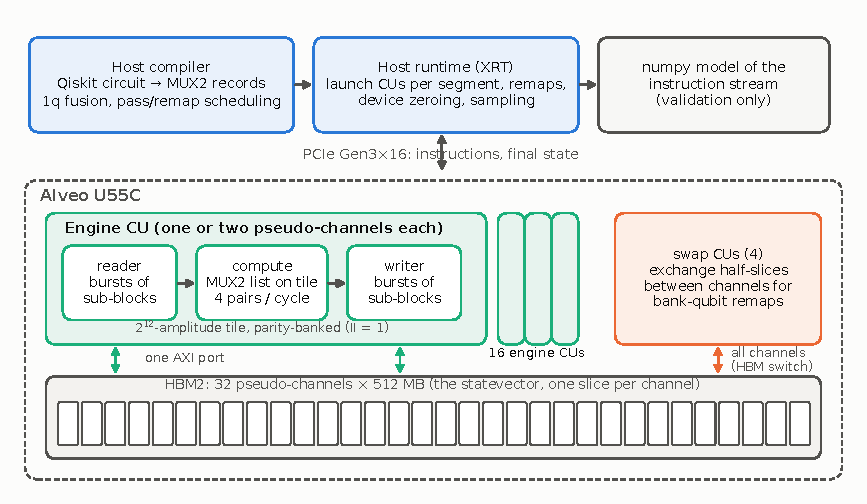
\includegraphics[width=\textwidth]{fig_architecture}
\caption{Revised simulator. The host compiler maps gates to MUX2 records, groups them into passes and encodes them; each engine compute unit (CU) owns the statevector slices of one or two HBM pseudo-channels and runs every pass as a reader, compute and writer dataflow pipeline over tiles; swap CUs exchange half-slices between pseudo-channels when a bank qubit must become local.}\label{fig:arch}
\end{figure}

\subsection{One datapath primitive for every gate}\label{subsec:mux2}

Every operation executed on the card is a \emph{multiplexed $2\times2$ update}, $\mathrm{MUX2}(t, C, M_0, M_1)$: for every amplitude pair $(a_{i}, a_{i\oplus 2^t})$ whose index has bit $t$ cleared, the engine applies $M_1$ if all qubits in the control set $C$ are 1 in $i$, and $M_0$ otherwise. The host maps gates to MUX2 records exactly:
\begin{itemize}
\item a single-qubit gate $U$ is $\mathrm{MUX2}(t,\emptyset,U,U)$; consecutive single-qubit gates on one qubit are multiplied into one record;
\item a controlled single-qubit gate (CX, CY, CH, CR$_{x,y,z}$, CSX, CS, CU, \ldots) is $\mathrm{MUX2}(t,\{c\},I,U)$, and multi-controlled gates (CCX, CCZ, MCX, MCPhase) use a larger control set;
\item a two-qubit diagonal gate (CZ, CP, R$_{zz}$) with diagonal $(d_0,d_1,d_2,d_3)$ is $\mathrm{MUX2}(b,\{a\},\mathrm{diag}(d_0,d_2),\mathrm{diag}(d_1,d_3))$;
\item any other two-qubit unitary (ECR, iSWAP, R$_{xx}$, R$_{yy}$, R$_{zx}$, XX$+$YY, DCX, \ldots) is written exactly as three MUX2 records using the cosine-sine decomposition $U=(L_0\oplus L_1)\,\mathrm{CS}\,(R_0\oplus R_1)$, where each block-diagonal factor is a MUX2 on one qubit controlled by the other;
\item SWAP is absorbed into the logical-to-physical qubit map and moves no data.
\end{itemize}
Only gates of three or more qubits that are not multi-controlled single-qubit gates (for example CSWAP), and multi-controlled gates wider than the tile window, are decomposed by Qiskit on the host. The engine therefore has a single arithmetic datapath: four amplitude pairs per cycle, each a $2\times2$ complex matrix-vector product in single precision (complex64), with per-pair selection between $M_0$ and $M_1$.

\subsection{Passes, tiles and on-chip banking}\label{subsec:tiles}

With $P$ active pseudo-channels the top $b=\log_2 P$ physical qubits select the PC (\emph{bank qubits}) and the remaining $L=n-b$ qubits index a contiguous slice inside it (\emph{local qubits}). A \emph{pass} streams the slice once: the reader gathers a tile of $2^{k}$ amplitudes ($k=12$), the compute stage applies an ordered list of up to 64 MUX2 records to the tile, and the writer stores it back. A tile consists of the $k-m$ lowest local qubits plus up to $m$ further \emph{high} local qubits $h_0,\ldots,h_{m-1}$; it is gathered as $2^m$ contiguous sub-blocks, each a long burst. Any gate whose qubits lie in this window is applied in the same pass, so a pass replaces several HBM sweeps. The build used for the main results supports $m\leq 4$ (\texttt{MAXH}$=4$); the earlier builds support $m\leq 2$.

Inside the engine a tile word $w$ (four amplitudes, 256~bits) is stored in bank $\mathrm{parity}(w)$ at address $\lfloor w/2\rfloor$. Two words whose indices differ in exactly one bit are always in different banks, so every pair update reads one word from each bank and writes one word to each bank per cycle. This gives an initiation interval of one for every target qubit without the runtime bank multiplexing that limited the baseline.

\subsection{Compute units, exchange and capacity}\label{subsec:cus}

Each engine is a separate compute unit with one AXI port to its own PC (or pair of PCs); the instructions of a pass are stored behind the state slice in the same buffer, because the HBM subsystem offers \NumHbmPortConnections{} port connections in total. A single kernel with 32 HBM ports could not be implemented: our first attempts at a 32-port microbenchmark exceeded the block RAM of the HBM-adjacent super logic region (\NumHbmFirstBramPct\,\%) and then failed routing (congestion level \NumHbmCongestion). Compute units are therefore spread over the three super logic regions.

When a gate acts on a bank qubit, the host remaps that qubit with a local one. The remap is executed on the card by \emph{swap} CUs whose two ports reach all 32 PCs through the HBM switch; it exchanges contiguous half-slices (or larger chunks) between the two PCs of each pair. Device-to-device buffer copies through XRT are not available on this shell (the M2M test reports ``not available'' and copies fall back to the host), and PCIe moves only \NumPcieHtoD~GB/s (host to card) and \NumPcieDtoH~GB/s (card to host), so a host-mediated remap of a 30-qubit state would cost seconds.

A slice must fit in one 512~MB PC together with its instructions for the swap CUs to address it. The main build therefore gives each engine two PCs and treats the statevector as up to 32 \emph{virtual slices} of one PC each, processed by 16 engines; this holds a 30-qubit complex64 state (8~GB) on one card while keeping all exchanges on the card. The host chooses the number of slices from the measured trade-off between kernel parallelism and remap cost (Section~\ref{subsec:res-ablation}).

\subsection{Host compiler and runtime}\label{subsec:host}

The host compiler (Python) converts a Qiskit circuit into MUX2 records, fuses consecutive single-qubit gates, and schedules passes greedily: a gate joins the open pass if the union of qubits still fits the tile window with at most $m$ high qubits, otherwise the pass is closed. A bank qubit, or a gate that needs more than $m$ high qubits, triggers a remap that prefers to swap bank qubits with high local qubits so that exchanged chunks stay large. The runtime launches all engine CUs for each segment of passes, executes remaps between segments, zeroes the state on the card instead of uploading it, and samples measurement outcomes directly from the per-slice buffers. A numpy model of the exact instruction stream is used to validate the compiler and the HLS C model before every build.

\begin{table}
\centering
\caption{Implemented builds (post-route). All engines are the same HLS source; builds differ in the number of engine CUs, PCs per engine, AXI width and the maximum number of high qubits per pass.}\label{tab:builds}
\footnotesize\setlength{\tabcolsep}{3pt}
\begin{tabular}{lrrrrrrrrr}
\toprule
Build & Engines & PCs & AXI bits & $m_\mathrm{max}$ & MHz & LUT & BRAM & URAM & DSP \\
\midrule
sv\_e8 & 8 & 8 & 256 & 2 & 300 & 225k (20\%) & 548 (30\%) & 64 & 2368 (26\%) \\
sv\_e16 & 16 & 16 & 256 & 2 & 298 & 420k (37\%) & 916 (50\%) & 64 & 4736 (53\%) \\
sv\_e16w & 16 & 32 & 256 & 2 & 298 & 420k (37\%) & 916 (50\%) & 64 & 4736 (53\%) \\
sv\_e16w512 & 16 & 32 & 512 & 2 & 288 & 454k (41\%) & 1028 (57\%) & 64 & 4736 (53\%) \\
sv\_e16w\_m4 & 16 & 32 & 256 & 4 & 300 & 448k (40\%) & 916 (50\%) & 64 & 4736 (53\%) \\
\bottomrule
\end{tabular}
\end{table}
%==========================================================================
\section{Experimental Methodology}\label{sec:methodology}

\subsection{Timing definitions}\label{subsec:timing}

Table~\ref{tab:timing} defines the timing fields used for every platform, table and figure in this paper. Per-circuit times exclude $T_\mathrm{setup}$. Each caption states which field it reports.

\begin{table}
\centering
\caption{Timing definitions (all platforms).}\label{tab:timing}
\small
\begin{tabular}{p{1.5cm}p{8.3cm}p{1.8cm}}
\toprule
Field & Definition & Scope \\
\midrule
$T_\mathrm{setup}$ & one-time: bitstream load, XRT/CUDA context, buffer allocation, imports & reported separately; excluded \\
$T_\mathrm{compile}$ & host transpile/lowering, fusion, pass scheduling, instruction encoding & per circuit \\
$T_\mathrm{h2d}$ & host-to-device transfer of instructions and initial state (FPGA: device zeroing pass + 32-byte write) & per circuit \\
$T_\mathrm{kernel}$ & device execution only (FPGA: XRT start to completion of all CUs; GPU: backend run; CPU: compute loop) & per circuit \\
$T_\mathrm{exch}$ & FPGA only: bank-qubit remaps between pseudo-channels or cards & per circuit \\
$T_\mathrm{d2h}$ & device-to-host transfer of the final state & per circuit \\
$T_\mathrm{post}$ & host sampling of 1,024 shots (fidelity checks excluded) & per circuit \\
$T_\mathrm{e2e}$ & $T_\mathrm{compile}+T_\mathrm{h2d}+T_\mathrm{kernel}+T_\mathrm{exch}+T_\mathrm{d2h}+T_\mathrm{post}$ & per circuit \\
\bottomrule
\end{tabular}
\end{table}

For the FPGA, $T_\mathrm{kernel}$ is the host-measured interval from starting all engine CUs of a segment to the completion of the last one, summed over segments; remaps are reported separately as $T_\mathrm{exch}$. For Qiskit Aer (CPU and GPU) the backend returns the statevector in host memory, so the measured run interval includes the state transfer and is reported as $T_\mathrm{kernel}$ with $T_\mathrm{d2h}=0$; we state this wherever Aer GPU numbers appear. The same boundary therefore applies to Aer on the CPU and on the GPU.

\subsection{Platforms and software}\label{subsec:platforms}

Table~\ref{tab:hwconfig} lists the platforms; versions were captured by script at measurement time. The CPU host is a dual-socket AMD EPYC 7742 server (2$\times$64 cores, 503~GiB). GPU measurements were made on an NVIDIA A100 SXM4 (80~GiB) in a node of a Slurm cluster, with the scripts and circuits used here; the RTX A4000 workstation of the submitted manuscript was not available for remeasurement, and no GPU number of the submitted manuscript is reused. Qiskit Aer (single and double precision, with and without cuStateVec) was run for all four families and CUDA-Q (single and double precision, \texttt{nvidia} target) for GHZ and QFT; the CUDA-Q jobs for RQC and VQE were cancelled by the cluster before they started and could not be repeated, and the widest widths that completed are given in Section~\ref{subsec:res-xplat}. The GPU timing fields do not involve the host processor except $T_\mathrm{compile}$, which is reported separately. No number from the submitted manuscript is reused.

\begin{table}
\centering
\caption{Hardware and software configuration (captured by \texttt{scripts/capture\_env.sh}).}\label{tab:hwconfig}
\small
\begin{tabular}{p{2.6cm}p{9.0cm}}
\toprule
FPGA/CPU host & 2 $\times$ AMD EPYC 7742 64-Core Processor (64 cores each), 503 GiB, Ubuntu 20.04.6 LTS \\
FPGA & AMD Alveo U55C, shell xilinx\_u55c\_gen3x16\_xdma\_base\_3, XRT 2.16.204, Vitis 2023.2 \\
FPGA host software & Python 3.8.20, NumPy 1.24.4, Qiskit 1.2.4 \\
CPU simulators & Qiskit Aer 0.17.2 (Qiskit 2.5.2), qsimcirq 0.22.1, Qulacs 0.6.14, Python 3.11.16 \\
GPU host & Slurm cluster node, 2 sockets $\times$ 32 cores (2 threads per core), 1007 GiB, Linux 5.14.0-737.el9.x86\_64 \\
GPU & NVIDIA A100-SXM4-80GB, 80 GiB, driver 615.71.09 \\
GPU simulators & Qiskit Aer GPU 0.15.1 with cuStateVec (cuQuantum 26.9.0), CUDA-Q 0.12.0 (nvidia target), Qiskit 1.2.4 \\
\bottomrule
\end{tabular}
\end{table}

\subsection{Benchmark circuits and protocol}\label{subsec:protocol}

We use the same four circuit families as the submitted manuscript, now generated with fixed seeds and exported as OpenQASM~\cite{cross2017openqasm}: GHZ (Hadamard plus a CX chain over all qubits), QFT with final swaps, random brick-wall circuits (RQC; random $R_x$, $R_y$, $R_z$, $T$ or $H$ on every qubit per layer followed by CZ on alternating pairs, depths 8, 10, 16 and 20) and a hardware-efficient VQE ansatz ($R_y R_z$ layers with a CX ladder, two layers), plus Grover search for $n\leq 12$~\cite{grover1996fast,peruzzo2014variational,boixo2018characterizing}. All platforms run identical circuit instances. Each point is the median of 10 repetitions ($n\leq 24$) or 3 repetitions ($n\geq 26$) after one warm-up run, on every platform; the inter-quartile range is reported where it is visible. The single-threaded NumPy simulator of the submitted manuscript, kept only as a legacy reference, was timed twice per point because of its run time. Every timed FPGA run returns the final state to host memory and samples 1{,}024 shots; CPU and GPU runs return the final statevector in host memory and do not sample. CPU runs were made with no other jobs on the host. FPGA runs on two cards were made concurrently, each in its own host process pinned to 16 cores of the NUMA node that hosts the card and limited to 8 math-library threads, with the host otherwise idle.

\subsection{Correctness}\label{subsec:correctness-method}

Correctness is checked independently of the benchmarks by a functional suite in which every gate test starts from a generic entangled state (a random $U_3$ layer, a ring of CZ gates and a second $U_3$ layer), so that no test can pass on the norm alone. The suite covers every single-qubit gate on every position, 21 two-qubit gates on every ordered pair, three- and four-qubit gates, the circuit families for $n=2$ to 20, and analytic checks of GHZ and QFT$|0\rangle$ states up to $n=30$. A case passes when $1-F\leq 10^{-5}$ with $F=|\langle\psi_\mathrm{ref}|\psi\rangle|^2/\langle\psi|\psi\rangle$ against a complex128 Qiskit reference. Inner products are accumulated in double precision. Beyond the suite, the full final state of every family at $n=24$ to 30 is compared with a complex128 Qiskit Aer statevector (gate fusion off) computed on the host after the card runs; the infidelity is computed without cancellation as $1-F=d^2-d^4/4$, where $d$ is the $\ell_2$ distance between the normalised states after optimal global-phase alignment.

\subsection{Energy}\label{subsec:energy-method}

Card power is read from the Alveo XMC sensors through sysfs (sum of the 12~V PCIe, 12~V auxiliary and 3.3~V PCIe rails, identical to the value reported by \texttt{xbutil}). The sensors refresh about once per second (\NumXmcPeriod~s measured), so energy is not integrated over single short runs: each circuit is repeated for at least 30~s and the time-weighted mean board power over the loop is multiplied by the per-run time. GPU power is read with \texttt{nvidia-smi} every 100~ms. We report two boundaries consistently for all platforms: \emph{device only} (card or GPU board power) and \emph{device plus host CPU package}. The CPU package energy counters (RAPL) are readable only with root privileges on the host used here, so the second boundary could not be measured and is not reported; PCIe switch, fans, cooling and power-supply losses are excluded on every platform. The analytical Alveo power model used in the submitted manuscript is compared against these measurements in Section~\ref{subsec:res-energy}.

During the 30-qubit runs a card reached the conservative abort limit we set (90\,$^\circ$C FPGA / 85\,$^\circ$C HBM) and the run was stopped automatically. Heavy runs were subsequently paced so that each repetition starts below a per-card temperature threshold; the waiting time is recorded with every result and excluded from all reported times.
%==========================================================================
\section{Results}\label{sec:results}

\subsection{Memory-system ceilings}\label{subsec:res-ceilings}

Table~\ref{tab:hbm} reports the streaming microbenchmark. One AXI port sustains \NumHbmSixteenPerCURead~GB/s when reading, \NumHbmSixteenPerCUWrite~GB/s when writing and \NumHbmSixteenPerCUCopy~GB/s for concurrent reading and writing of one pseudo-channel, for 256- and 512-bit ports alike; the vendor's validation kernel reaches \NumHbmVendorOneBank~GB/s on one bank. Bandwidth scales linearly with the number of active channels, whether the active channels are adjacent or spread over both HBM stacks, up to \NumHbmSixteenCopy~GB/s on 16 channels and \NumHbmThirtytwoCopy~GB/s on all 32 channels in copy mode (\NumHbmThirtytwoRead~GB/s read-only, limited there by the 256-bit ports of that build). The practical ceiling of the card is therefore \NumHbmCeilingPct\,\% of the nominal 460~GB/s, and one channel, not the switch or the controller, is the unit of bandwidth. PCIe moves \NumPcieHtoD~GB/s to the card and \NumPcieDtoH~GB/s back.

Figure~\ref{fig:roofline} places the revised kernel on a roofline built from these measurements. Each MUX2 pair update costs 28 floating-point operations and 32~bytes per pass, so the arithmetic intensity of a pass grows with the number of gates it applies. The engines' compute peak (16 engines, four pair updates per cycle at \NumFlagClockMHz~MHz) is \NumFlagComputeRoof~GFLOP/s. GHZ, whose passes contain few gates, stays below the 16-channel bandwidth roof; QFT, RQC and VQE, whose passes contain many gates, run close to the compute peak.

\begin{table}
\centering
\caption{Measured HBM bandwidth on the U55C (streaming microbenchmark, one AXI port per CU, 128~MiB per CU per repetition, median of 5). ``Per CU'' is one active CU; the last column uses all CUs of the build.}\label{tab:hbm}
\small
\begin{tabular}{llrrr}
\toprule
Build & Mode & 1 CU (GB/s) & CUs & All CUs (GB/s) \\
\midrule
16 CUs $\times$ 512-bit & read & 12.8 & 16 & 202.6 \\
16 CUs $\times$ 512-bit & write & 12.8 & 16 & 201.7 \\
16 CUs $\times$ 512-bit & copy & 12.6 & 16 & 201.4 \\
32 CUs $\times$ 256-bit & read & 9.4 & 32 & 294.1 \\
32 CUs $\times$ 256-bit & write & 9.0 & 32 & 280.9 \\
32 CUs $\times$ 256-bit & copy & 12.6 & 32 & 398.9 \\
\bottomrule
\end{tabular}
\end{table}

\begin{figure}
\centering
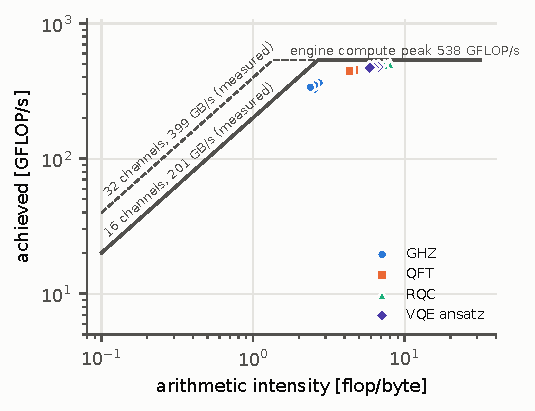
\includegraphics[width=\textwidth]{fig_roofline}
\caption{Roofline of the revised kernel (build sv\_e16w\_m4, $n=26$ to 30, $T_\mathrm{kernel}$). Roofs are measured (bandwidth) or derived from the build (compute: 16 engines $\times$ 4 pair updates per cycle $\times$ 28~flop). Points: one per circuit and size; arithmetic intensity is 28/32 times the mean number of gates per pass.}\label{fig:roofline}
\end{figure}

\subsection{Correctness}\label{subsec:res-correct}

\begin{table}
\centering
\caption{Gate support in four categories (R1.1): (a) native in the kernel, (b) native and verified by the functional suite, (c) supported through host lowering, (d) not supported or failing.}\label{tab:gates}
\small
\begin{tabular}{p{2.6cm}p{4.4cm}p{4.4cm}}
\toprule
Category & Baseline (v07) & Revised kernel \\
\midrule
(a) native in the kernel & 19 opcodes: I, H, X, Y, Z, S, T, S$^\dagger$, T$^\dagger$, $\sqrt{X}$, $\sqrt{X}^\dagger$, R$_x$, R$_y$, R$_z$, P, U2, U3, CX, CZ & one primitive, MUX2 (multiplexed $2\times2$ on one target, optional controls) \\
(b) native and verified by test & I, H, X, Y, Z, S, T, S$^\dagger$, T$^\dagger$, $\sqrt{X}$, $\sqrt{X}^\dagger$, R$_x$, R$_y$, R$_z$, P, U, CX, CZ & all gates of (c) below, executed as 1 to 3 MUX2 records; 43 gate types verified \\
(c) supported via host lowering & CCX, CH, CP, CR$_x$, CR$_y$, CR$_z$, CSX, CY, DCX, ECR, iSWAP, MCX (3 controls), MCX (4 controls), R$_{xx}$, R$_{yy}$, R$_{zz}$, SWAP (exact lowerings to 1q+CX+CZ) & none lowered to other gates; 2q non-controlled gates use the exact cosine-sine form (3 MUX2); SWAP is a relabel; gates wider than the tile window are decomposed by Qiskit \\
(d) not supported / failing & CCZ, CS, CS$^\dagger$, CSWAP, CU, R, R$_{zx}$, XX+YY & none \\
\bottomrule
\end{tabular}
\end{table}

\begin{table}
\centering
\caption{Functional suite: cases passing $1-F\leq 10^{-5}$ (revised kernel) and $1-F\leq 10^{-10}$ (complex128 baseline) against a complex128 Qiskit reference; every gate test starts from a generic entangled state.}\label{tab:suite}
\small
\begin{tabular}{lrr}
\toprule
Section & Baseline (v07) & Revised \\
\midrule
single-qubit gates (17 gates $\times$ 5 positions) & 80/85 & 85/85 \\
two-qubit gates (21 gates $\times$ 12 ordered pairs) & 192/252 & 252/252 \\
three- and more-qubit gates & 4/7 & 7/7 \\
circuit families, $n=2$ to 20 & 46/46 & 46/46 \\
analytic large-$n$ checks & 6/6 & 8/8 \\
\midrule
Total & 328/396 & 398/398 \\
\bottomrule
\end{tabular}
\end{table}

Table~\ref{tab:gates} replaces the gate table of the submitted manuscript. The baseline kernel implemented \NumVsevenOpcodes{} opcodes and relied on host lowering for every other gate; \NumVsevenUnsupportedTypes{} gate types of the suite were not supported. The revised kernel has one native primitive, and every gate type of the suite is executed through it. On the functional suite (Table~\ref{tab:suite}) the revised simulator passes all \NumSuiteTotal{} cases on every build tested, including GHZ and QFT checks at 24 to 30 qubits; the largest infidelity among the gate tests is $\NumSuiteWorstInfNew$, at the single-precision level. The baseline passes \NumSuitePassVseven{} of \NumSuiteTotalVseven{} cases at the tighter $10^{-10}$ threshold its complex128 arithmetic allows; all of its failures are unsupported gates.

\textbf{Largest width on one card.} One card holds at most 30 qubits in complex64. The state of $2^{30}$ amplitudes occupies \NumMaxwStateGiB~GiB, stored as 32 single-channel slices of 256~MiB, each followed by the instruction region of its engine in the same buffer; a 31-qubit state (16~GiB) would fill every pseudo-channel completely and leave no room for the instructions. To verify the simulator at this limit, every circuit family was run at $n=24$ to 30 on one card and its full final state compared with a complex128 Qiskit Aer reference computed on the host (Table~\ref{tab:maxwidth}, Fig.~\ref{fig:maxwidth}). At $n=\NumMaxwN$ all \NumMaxwFamilies{} families agree with the reference to $1-F\leq\NumMaxwWorstInfThirty$; over all widths the largest infidelity is $\NumMaxwWorstInf$ and the largest amplitude error $\NumMaxwWorstAbs$, the level expected from single-precision arithmetic.

\begin{figure}
\centering
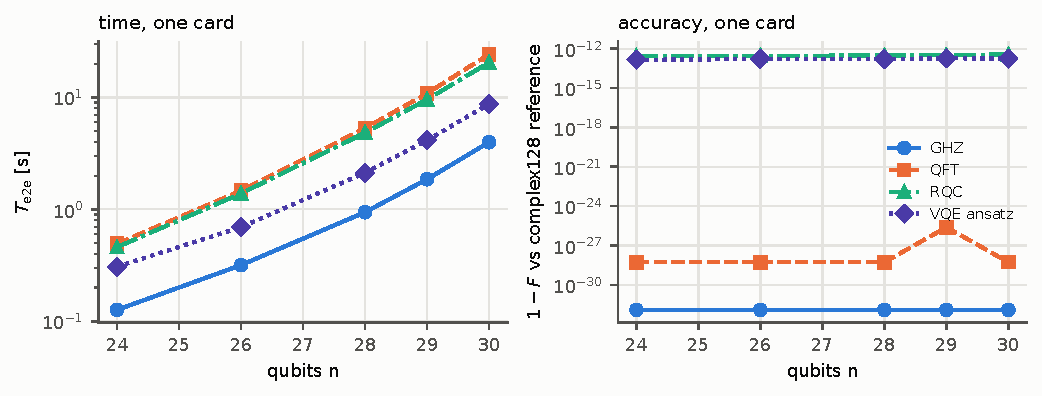
\includegraphics[width=\textwidth]{fig_maxwidth}
\caption{Largest widths on one card (build sv\_e16w\_m4, one run per point after a warm-up run): end-to-end time (left) and infidelity of the full final state against a complex128 Qiskit Aer reference (right). GHZ is exact to double-precision rounding at every width.}\label{fig:maxwidth}
\end{figure}

\begin{table}
\centering
\caption{Verification at the largest widths on one card (build sv\_e16w\_m4): number of slices $P$, passes and remaps of the compiled circuit, $T_\mathrm{e2e}$ of the verified run, and infidelity and largest amplitude error after global-phase alignment against a complex128 Qiskit Aer statevector (gate fusion off). RQC has depth 10.}\label{tab:maxwidth}
\small
\begin{tabular}{lrrrrrrr}
\toprule
Circuit & $n$ & $P$ & passes & remaps & $T_\mathrm{e2e}$ (s) & $1-F$ & max $|\Delta a|$ \\
\midrule
GHZ & 24 & 16 & 8 & 4 & 0.126 & $1.2\times 10^{-32}$ & $1.1\times 10^{-16}$ \\
 & 26 & 16 & 9 & 4 & 0.318 & $1.2\times 10^{-32}$ & $1.1\times 10^{-16}$ \\
 & 28 & 16 & 9 & 4 & 0.943 & $1.2\times 10^{-32}$ & $1.1\times 10^{-16}$ \\
 & 29 & 16 & 10 & 4 & 1.86 & $1.2\times 10^{-32}$ & $1.1\times 10^{-16}$ \\
 & 30 & 32 & 11 & 5 & 3.98 & $1.2\times 10^{-32}$ & $1.1\times 10^{-16}$ \\
\addlinespace
QFT & 24 & 16 & 51 & 22 & 0.493 & $5.2\times 10^{-29}$ & $2.2\times 10^{-18}$ \\
 & 26 & 16 & 63 & 22 & 1.47 & $5.3\times 10^{-29}$ & $1.1\times 10^{-18}$ \\
 & 28 & 16 & 75 & 22 & 5.31 & $5.3\times 10^{-29}$ & $5.7\times 10^{-19}$ \\
 & 29 & 16 & 82 & 22 & 10.8 & $2.4\times 10^{-26}$ & $6.8\times 10^{-18}$ \\
 & 30 & 32 & 94 & 29 & 24.3 & $5.3\times 10^{-29}$ & $2.9\times 10^{-19}$ \\
\addlinespace
RQC & 24 & 16 & 39 & 18 & 0.459 & $2.8\times 10^{-13}$ & $2.7\times 10^{-9}$ \\
 & 26 & 16 & 42 & 18 & 1.39 & $2.8\times 10^{-13}$ & $2.1\times 10^{-9}$ \\
 & 28 & 16 & 46 & 18 & 4.83 & $3.0\times 10^{-13}$ & $1.9\times 10^{-9}$ \\
 & 29 & 16 & 46 & 18 & 9.57 & $3.2\times 10^{-13}$ & $1.4\times 10^{-9}$ \\
 & 30 & 32 & 52 & 23 & 20.5 & $3.7\times 10^{-13}$ & $1.4\times 10^{-9}$ \\
\addlinespace
VQE & 24 & 16 & 15 & 8 & 0.307 & $1.4\times 10^{-13}$ & $5.8\times 10^{-9}$ \\
 & 26 & 16 & 17 & 8 & 0.693 & $1.7\times 10^{-13}$ & $1.5\times 10^{-9}$ \\
 & 28 & 16 & 18 & 8 & 2.13 & $1.6\times 10^{-13}$ & $9.2\times 10^{-10}$ \\
 & 29 & 16 & 20 & 8 & 4.13 & $1.9\times 10^{-13}$ & $8.9\times 10^{-10}$ \\
 & 30 & 32 & 22 & 10 & 8.73 & $1.8\times 10^{-13}$ & $7.7\times 10^{-10}$ \\
\bottomrule
\end{tabular}
\end{table}

\subsection{Design-space study}\label{subsec:res-ablation}

\begin{table}
\centering
\caption{Ablations at $n=26$ (build \NumAblSource): $T_\mathrm{kernel}$ / $T_\mathrm{exch}$ in seconds and the number of passes in parentheses, median of 3.}\label{tab:ablation}
\footnotesize\setlength{\tabcolsep}{3pt}
\begin{tabular}{p{3.6cm}llll}
\toprule
Configuration & GHZ & QFT & RQC & VQE \\
\midrule
default ($k=12$, fusion, tiling, block layout, device exchange) & 0.07 / 0.07 (9) & 0.74 / 0.37 (63) & 0.73 / 0.31 (42) & 0.26 / 0.14 (17) \\
tile $k=9$ & 0.12 / 0.07 (10) & 1.27 / 0.37 (87) & 1.03 / 0.31 (47) & 0.38 / 0.15 (20) \\
tile $k=10$ & 0.09 / 0.07 (9) & 0.96 / 0.37 (79) & 0.85 / 0.31 (45) & 0.30 / 0.15 (18) \\
tile $k=11$ & 0.08 / 0.07 (9) & 0.80 / 0.37 (69) & 0.77 / 0.31 (44) & 0.27 / 0.15 (18) \\
no 1q fusion & 0.07 / 0.07 (9) & 0.75 / 0.36 (63) & 0.79 / 0.42 (59) & 0.39 / 0.07 (11) \\
one gate per pass & 0.15 / 0.07 (26) & 2.08 / 0.37 (351) & 2.20 / 0.31 (377) & 0.75 / 0.15 (128) \\
no fusion, one gate per pass & 0.15 / 0.07 (26) & 2.08 / 0.37 (351) & 2.25 / 0.42 (385) & 1.20 / 0.07 (206) \\
modulo-style initial layout & 0.08 / 0.08 (10) & 0.70 / 0.13 (61) & 0.73 / 0.15 (34) & 0.26 / 0.19 (19) \\
host-mediated exchange & 0.07 / 1.19 (9) & 0.75 / 6.06 (63) & 0.73 / 5.21 (42) & 0.26 / 2.32 (17) \\
\bottomrule
\end{tabular}
\end{table}

\textbf{Engines and channels.} Kernel time falls in proportion to the number of active engines (Fig.~\ref{fig:cu}): from one to eight engines it drops by \NumCuScaleOneToEight$\times$ on average over the four families, close to the ideal factor of eight, because every engine streams its own channel and the engines never share data within a pass. Doubling the engines from 8 to 16 lowers it by another \NumBuildEightToSixteen$\times$ at 28 qubits (geometric mean, Fig.~\ref{fig:builds}). Giving each engine a second channel does not change the kernel time (ratio \NumBuildSixteenToWide) but doubles the capacity, from \NumBuildSixteenMaxN{} to \NumBuildWideMaxN{} qubits, because an engine streams one channel at a time.

\textbf{Port width.} A 512-bit port does not raise the bandwidth of an engine while it streams one channel (Table~\ref{tab:hbm}); the 512-bit build used more logic and closed timing at a lower clock (Table~\ref{tab:builds}), so the main build keeps 256-bit ports.

\textbf{Passes, tiles and fusion.} Table~\ref{tab:ablation} isolates the host-side and tile-level optimisations at $n=26$. Applying all gates that fit a tile in one pass instead of one gate per pass reduces the kernel time by \NumAblTilingSpeedup$\times$ (geometric mean over the families) and the number of passes by up to an order of magnitude; fusing consecutive single-qubit gates adds \NumAblFusionSpeedup$\times$. Larger tiles reduce the number of passes because more qubits fit the window. Allowing four instead of two high qubits per tile roughly halves the passes of QFT, RQC and VQE (builds sv\_e16w and sv\_e16w\_m4 in Fig.~\ref{fig:builds}).

\textbf{Exchange and layout.} Executing remaps on the card instead of through host memory lowers the exchange time by \NumAblSwapSpeedup$\times$. The initial placement of qubits matters little because remapping adapts it; a modulo-style placement, which starts with the lowest logical qubits on the bank positions, even reduces the number of remaps for QFT and RQC.

\begin{figure}
\centering
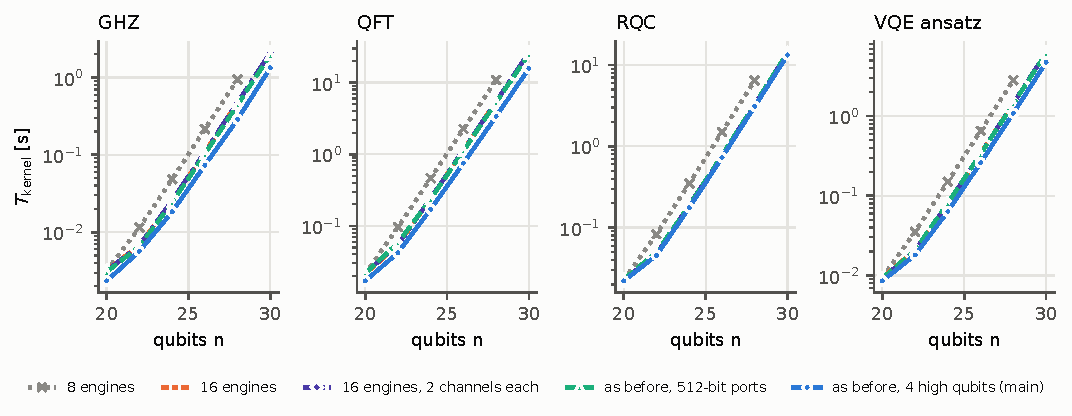
\includegraphics[width=\textwidth]{fig_builds}
\caption{Kernel time of the five builds of Table~\ref{tab:builds} on the same circuits ($T_\mathrm{kernel}$, median of 3, $n=20$ to 30 as far as each build's capacity allows).}\label{fig:builds}
\end{figure}

\begin{figure}
\centering
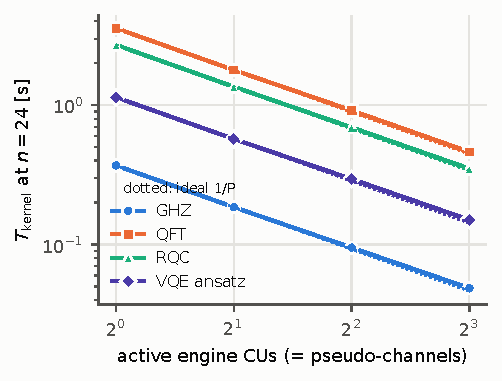
\includegraphics[width=0.48\textwidth]{fig_cu_scaling}
\caption{Kernel time versus the number of active engine CUs (build sv\_e8, $n=24$, median of 3); dotted lines show ideal $1/P$ scaling.}\label{fig:cu}
\end{figure}

\subsection{Scaling to 30 qubits on one card}\label{subsec:res-scaling}

\begin{figure}
\centering
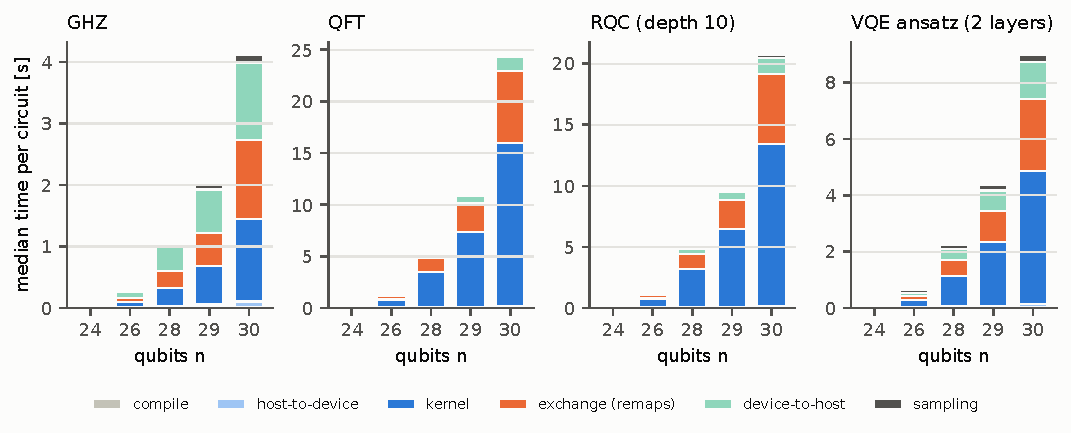
\includegraphics[width=\textwidth]{fig_breakdown}
\caption{Median time per circuit on one card (build sv\_e16w\_m4), split into the fields of Table~\ref{tab:timing}. At $n=30$ the state occupies 32 single-channel slices processed by 16 engines.}\label{fig:breakdown}
\end{figure}

Figure~\ref{fig:breakdown} shows the full time breakdown from 24 to 30 qubits on one card. GHZ-30 completes in \NumFlagGhzThirtyEtoE~s end to end (kernel \NumFlagGhzThirtyKernel~s), VQE-30 in \NumFlagVqeThirtyEtoE~s, RQC-30 in \NumFlagRqcThirtyEtoE~s and QFT-30 in \NumFlagQftThirtyEtoE~s. The kernel dominates for QFT and RQC; exchange accounts for \NumFlagQftThirtyExch~s of QFT-30 and \NumFlagGhzThirtyExch~s of GHZ-30 and is the largest remaining overhead; at 30 qubits the device-to-host transfer of the final state also becomes visible. Compared with the baseline on identical circuits, $T_\mathrm{e2e}$ at $n=24$ is \NumSpeedupVsevenGhzTwentyFour$\times$ lower for GHZ, \NumSpeedupVsevenVqeTwentyFour$\times$ for VQE, \NumSpeedupVsevenRqcTwentyFour$\times$ for RQC and \NumSpeedupVsevenQftTwentyFour$\times$ for QFT, and \NumSpeedupVsevenGhzTwentyEight$\times$ for GHZ-28. The effective HBM sweep rate at $n=30$, counting every pass as a full read and write of the state, is \NumFlagGhzThirtySweepBw~GB/s for GHZ and \NumFlagRqcThirtySweepBw to \NumFlagQftThirtySweepBw~GB/s for the circuits whose passes are compute-bound.

\subsection{Cross-platform comparison}\label{subsec:res-xplat}

\begin{figure}
\centering
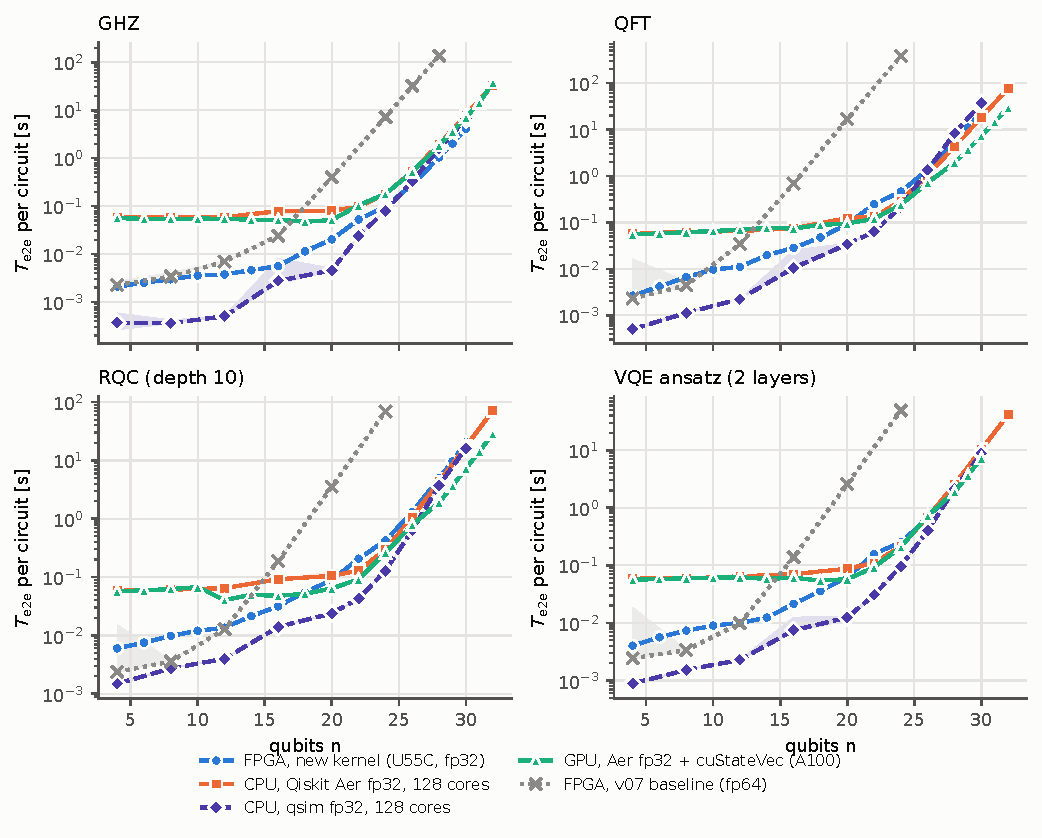
\includegraphics[width=\textwidth]{fig_xplat}
\caption{Median $T_\mathrm{e2e}$ per circuit on every platform (bands: inter-quartile range). FPGA: build sv\_e16w\_m4 on one U55C. CPU: dual EPYC 7742, 128 threads. Qiskit Aer and the GPU include the return of the state to host memory in their run time (Section~\ref{subsec:timing}).}\label{fig:xplat}
\end{figure}

\begin{table}
\centering
\caption{Median time per circuit in seconds at $n=24$, 28 and 30. FPGA: $T_\mathrm{kernel}$ and $T_\mathrm{e2e}$ of build sv\_e16w\_m4; CPU (128 threads) and GPU: $T_\mathrm{e2e}$. The ratio column divides the fastest of the six CPU configurations measured (Aer fp32 and fp64 with and without fusion, qsim, Qulacs) by the FPGA $T_\mathrm{e2e}$; values above 1 mean that the FPGA is faster. GPU: Qiskit Aer with cuStateVec and CUDA-Q on an NVIDIA A100 in a different host, $T_\mathrm{e2e}$ (Section~\ref{subsec:platforms}); CUDA-Q was measured for GHZ and QFT only.}\label{tab:xplat}
\footnotesize\setlength{\tabcolsep}{3pt}
\begin{tabular}{lrrrrrrrrrrr}
\toprule
 & & \multicolumn{2}{c}{FPGA} & \multicolumn{4}{c}{CPU, 128 threads} & best CPU & \multicolumn{3}{c}{GPU, A100} \\
\cmidrule(lr){3-4}\cmidrule(lr){5-8}\cmidrule(lr){10-12}
 & & & & \multicolumn{2}{c}{Aer} & qsim & Qulacs & / FPGA & \multicolumn{2}{c}{Aer} & CUDA-Q \\
Circuit & $n$ & kernel & e2e & fp32 & fp64 & fp32 & fp64 & e2e & fp32 & fp64 & fp32 \\
\midrule
GHZ & 24 & 0.0198 & 0.0992 & 0.179 & 0.128 & 0.0802 & 0.0469 & 0.47 & 0.180 & 0.217 & 0.133 \\
 & 28 & 0.289 & 1.04 & 1.98 & 1.30 & 1.61 & 1.26 & 1.21 & 1.85 & 2.09 & 1.13 \\
 & 30 & 1.34 & 4.11 & 7.91 & 5.28 & 6.58 & 5.17 & 1.21 & 7.16 & 8.09 & 4.30 \\
\addlinespace
QFT & 24 & 0.175 & 0.460 & 0.289 & 0.270 & 0.213 & 0.187 & 0.41 & 0.239 & 0.267 & 0.300 \\
 & 28 & 3.38 & 5.38 & 4.33 & 4.31 & 8.25 & 11.7 & 0.80 & 1.93 & 2.09 & 1.40 \\
 & 30 & 15.8 & 24.5 & 18.3 & 18.4 & 37.0 & 52.4 & 0.75 & 7.29 & 8.04 & 14.3 \\
\addlinespace
RQC & 24 & 0.177 & 0.423 & 0.297 & 0.281 & 0.129 & 0.304 & 0.31 & 0.262 & 0.237 & n/a \\
 & 28 & 3.11 & 4.94 & 4.32 & 3.78 & 3.75 & 12.5 & 0.76 & 1.90 & 2.09 & n/a \\
 & 30 & 13.3 & 20.7 & 17.3 & 15.7 & 16.2 & 55.2 & 0.76 & 7.24 & 7.99 & n/a \\
\addlinespace
VQE & 24 & 0.0641 & 0.252 & 0.216 & 0.161 & 0.0968 & 0.195 & 0.38 & 0.208 & 0.230 & n/a \\
 & 28 & 1.08 & 2.25 & 2.56 & 1.83 & 2.12 & 8.88 & 0.81 & 1.89 & 2.06 & n/a \\
 & 30 & 4.74 & 8.98 & 10.3 & 7.52 & 8.79 & 37.8 & 0.84 & 7.28 & 7.99 & n/a \\
\bottomrule
\end{tabular}
\end{table}

Figure~\ref{fig:xplat} and Table~\ref{tab:xplat} compare the revised simulator with three CPU simulators on a dual-socket server whose memory sustains \NumCpuTriad~GB/s in the STREAM triad, and with a GPU. The comparison is end to end: the FPGA time includes compilation of the circuit on the host, the transfer of the instructions, all passes and remaps, the return of the final state to host memory and the sampling of 1{,}024 shots; the CPU time includes the simulator's own transpilation and leaves the final state in host memory without sampling. At 30 qubits the state return and sampling add about \NumFlagDtwohGhzThirty~s and \NumFlagPostGhzThirty~s to the FPGA time of GHZ, so the comparison is conservative for the FPGA.

For small and medium circuits the FPGA is slower than the fastest CPU simulator. A circuit of four qubits takes \NumXplatFpgaSmallMs~ms on the card (median over the families), almost all of it fixed host-side and launch overhead, against \NumXplatCpuSmallUs~$\mu$s for the fastest CPU simulator; at 24 qubits the best CPU configuration needs \NumXplatRatioTwentyFourMin to \NumXplatRatioTwentyFourMax{} of the FPGA time. From \NumXplatGhzCrossN{} qubits upwards GHZ, whose passes carry few gates and are bound by HBM bandwidth, runs faster on the FPGA than on any CPU configuration, by a factor of \NumXplatRatioGhzThirty{} at 30 qubits. For QFT, RQC and VQE the 128-core server remains faster at every size: the best CPU configuration needs \NumXplatRatioQftThirty, \NumXplatRatioRqcThirty{} and \NumXplatRatioVqeThirty{} of the FPGA time at 30 qubits. These circuits have many gates per pass and are bound by the arithmetic of the 16 engines (Fig.~\ref{fig:roofline}). The CPU result depends strongly on the simulator and its settings: no single CPU configuration is fastest at every size, and at 30 qubits the fastest is \NumXplatBestCpuGhzThirty{} for GHZ, \NumXplatBestCpuQftThirty{} for QFT, \NumXplatBestCpuRqcThirty{} for RQC and \NumXplatBestCpuVqeThirty{} for VQE. Against Aer in single precision with fusion, the configuration closest to the FPGA's arithmetic, the time ratio at 30 qubits is \NumXplatAerRatioGhzThirty{} for GHZ, \NumXplatAerRatioQftThirty{} for QFT, \NumXplatAerRatioRqcThirty{} for RQC and \NumXplatAerRatioVqeThirty{} for VQE.

The GPU reference is an NVIDIA A100 (80~GiB HBM2e) of a cluster node, a different host from the FPGA and CPU
measurements (Section~\ref{subsec:platforms}), running Qiskit Aer with cuStateVec on all four families and CUDA-Q on GHZ and QFT, with the same circuits and
seeds. The A100 holds up to \NumGpuMaxN~qubits with Aer and \NumGpuCudaqSingleMaxN~qubits with CUDA-Q in single precision,
beyond the 30 qubits of one U55C. At 30 qubits the Aer times are almost the same for every family
(\NumXplatGpuTGhzThirty~s for GHZ, \NumXplatGpuTQftThirty~s for QFT): Aer reports \NumGpuAerTimeThirtyMin~to
\NumGpuAerTimeThirtyMax~s of simulation, and the rest is the return of the 8~GiB state to host memory, which the FPGA time
also contains (\NumFlagDtwohGhzThirty~s for GHZ). Against the fastest GPU configuration of each family at 30 qubits, the GPU
is faster than the card by a factor of \NumXplatBestGpuRatioQftThirty~for QFT, \NumXplatBestGpuRatioRqcThirty~for RQC and
\NumXplatBestGpuRatioVqeThirty~for VQE. For GHZ, whose passes are bound by HBM bandwidth, the two are about equal: the
fastest GPU configuration (\NumXplatBestGpuNameGhzThirty) needs \NumXplatBestGpuTGhzThirty~s against \NumFlagGhzThirtyEtoE~s on
the card, a time ratio of \NumXplatBestGpuRatioGhzThirty. Without cuStateVec Aer is slower by a factor of
\NumGpuCusvGainGhzThirty~(GHZ) and \NumGpuCusvGainQftThirty~(QFT). In double precision Aer needs \NumGpuAerDoubleTGhzThirty~s
for GHZ and \NumGpuAerDoubleTQftThirty~s for QFT at 30 qubits, close to its single-precision times because the state return
dominates; its 32-qubit double-precision runs returned no state. The GPU used Qiskit Aer 0.15.1 and CUDA-Q 0.12.0, the CPU
Aer 0.17.2 (Table~\ref{tab:hwconfig}).

\subsection{Energy}\label{subsec:res-energy}

\begin{table}
\centering
\caption{Measured card power and energy per circuit at the device boundary (sustained loops of at least \NumEnergyLoopS~s, revised kernel sv\_e16w\_m4; the baseline where it ran). $E = \bar P\,t$; EDP $= E\,t$.}\label{tab:energy}
\small
\begin{tabular}{lrrrrrrr}
\toprule
 & & \multicolumn{4}{c}{Revised kernel} & \multicolumn{2}{c}{Baseline (v07)} \\
\cmidrule(lr){3-6}\cmidrule(lr){7-8}
Circuit & $n$ & $t$ (s) & $\bar P$ (W) & $E$ (J) & EDP (J\,s) & $E$ (J) & ratio \\
\midrule
GHZ & 20 & 0.0206 & 39.2 & 0.807 & 0.0166 & 10.7 & 13 \\
 & 24 & 0.101 & 40.3 & 4.08 & 0.413 & 197 & 48 \\
 & 26 & 0.277 & 41.0 & 11.4 & 3.14 & n/a & n/a \\
 & 28 & 1.04 & 42.4 & 44.0 & 45.6 & n/a & n/a \\
 & 30 & 4.19 & 43.4 & 182 & 761 & n/a & n/a \\
\addlinespace
QFT & 20 & 0.0919 & 39.2 & 3.61 & 0.332 & n/a & n/a \\
 & 24 & 0.460 & 41.1 & 18.9 & 8.70 & n/a & n/a \\
 & 26 & 1.36 & 42.9 & 58.2 & 78.9 & n/a & n/a \\
 & 28 & 5.41 & 44.5 & 241 & 1305 & n/a & n/a \\
 & 30 & 24.5 & 44.4 & 1088 & 26621 & n/a & n/a \\
\addlinespace
RQC & 20 & 0.0864 & 40.2 & 3.47 & 0.299 & 95.5 & 28 \\
 & 24 & 0.428 & 43.7 & 18.7 & 7.99 & 1862 & 100 \\
 & 26 & 1.29 & 43.5 & 56.2 & 72.6 & n/a & n/a \\
 & 28 & 4.94 & 47.8 & 236 & 1165 & n/a & n/a \\
 & 30 & 20.7 & 48.3 & 999 & 20684 & n/a & n/a \\
\addlinespace
VQE & 20 & 0.0613 & 39.6 & 2.43 & 0.149 & 68.1 & 28 \\
 & 24 & 0.253 & 42.4 & 10.7 & 2.72 & 1298 & 121 \\
 & 26 & 0.650 & 44.0 & 28.6 & 18.6 & n/a & n/a \\
 & 28 & 2.24 & 46.4 & 104 & 232 & n/a & n/a \\
 & 30 & 8.92 & 51.9 & 462 & 4125 & n/a & n/a \\
\bottomrule
\end{tabular}
\end{table}

Table~\ref{tab:energy} reports the measured board power and energy. The card draws \NumFlagPowerMin to \NumFlagPowerMax~W while the revised kernel runs, against \NumVsevenPowerMin to \NumVsevenPowerMax~W for the baseline, whose engines are mostly waiting for memory. Because the run time falls by far more than the power rises, the energy per circuit is \NumEnergyVsevenRatioMin to \NumEnergyVsevenRatioMax{} times lower than with the baseline. At 30 qubits a GHZ circuit costs \NumFlagEnergyGhzThirty~J and a QFT \NumFlagEnergyQftThirty~J at the device boundary.

The analytical power model of the submitted manuscript predicts \NumModelPowerW~W for the baseline. Against the measured runs the model overestimates power by \NumModelPowerErrMin to \NumModelPowerErrMax\,\% and energy by \NumModelEnergyErrMin to \NumModelEnergyErrMax\,\%; the energy error is larger because the model's cycle estimate also exceeds the measured kernel time. We therefore no longer use the model and report only measured values.

The CPU server's package power could not be read (Section~\ref{subsec:energy-method}), so no CPU energy is reported. The A100 draws \NumGpuPowerMin~to \NumGpuPowerMax~W of board power during the 30 qubit runs,
from at least \NumGpuPowerReadingsMin~readings per run; its energy per circuit at 30 qubits is \NumGpuEnergyGhzThirty~J for
GHZ and \NumGpuEnergyQftThirty~J for QFT, against \NumFlagEnergyGhzThirty~J and \NumFlagEnergyQftThirty~J for the FPGA.
The GPU values are integrated over single runs rather than sustained loops, which the 100~ms sampling of the GPU sensor
allows at this length.

\subsection{Latency distribution}\label{subsec:res-jitter}

\begin{figure}
\centering
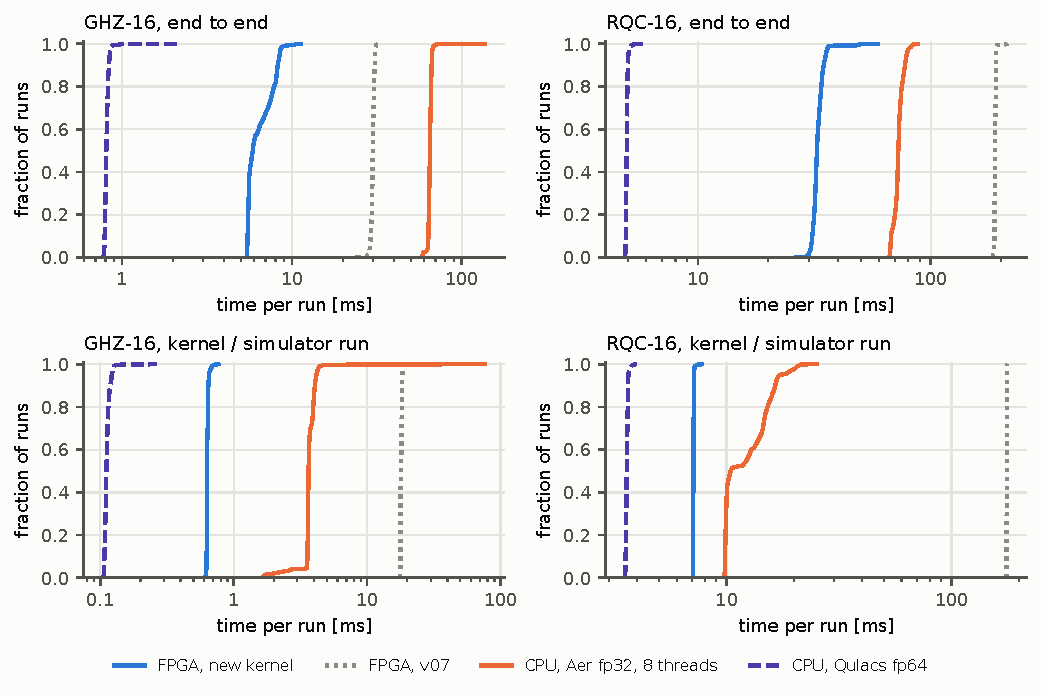
\includegraphics[width=\textwidth]{fig_jitter}
\caption{Distribution of the time per run over 2{,}000 runs of GHZ-16 and RQC-16 (after 20 warm-up runs), end to end (top) and kernel or simulator run only (bottom).}\label{fig:jitter}
\end{figure}

For small circuits run many times, as in variational loops, the spread of the run time matters as much as its median. Over 2{,}000 runs at 12 and 16 qubits (Fig.~\ref{fig:jitter}) the kernel time of the revised simulator varies little: its 99th percentile exceeds the median by \NumJitterKSvSpreadMin to \NumJitterKSvSpreadMax\,\%, similar to the baseline kernel (\NumJitterKVsevenSpreadMin to \NumJitterKVsevenSpreadMax\,\%) and tighter than the simulator run of Qiskit Aer on 8 CPU threads (\NumJitterKAerSpreadMin to \NumJitterKAerSpreadMax\,\%) and Qulacs (\NumJitterKQulacsSpreadMin to \NumJitterKQulacsSpreadMax\,\%). End to end the picture reverses: the FPGA path varies by \NumJitterSvSpreadMin to \NumJitterSvSpreadMax\,\% over all sizes, against \NumJitterAerSpreadMin to \NumJitterAerSpreadMax\,\% for Aer, because its time is dominated by host-side compilation, buffer synchronisation and kernel launches. The hardware is deterministic, but an application sees that only if its host path is equally predictable. No latency
distribution was measured on the GPU.
%==========================================================================
\section{Discussion}\label{sec:discussion}

The measurements separate three regimes.

\textbf{Where the FPGA wins.} Circuits whose passes carry few gates per amplitude, such as GHZ, are bound by memory bandwidth. Here 16 engines streaming their own channels outrun a 128-core server from \NumXplatGhzCrossN{} qubits upwards, even though the FPGA time includes returning the state to the host and sampling, work the CPU runs do not do. Against the baseline kernel on the same card the redesign is faster and more energy-efficient at every size, because the baseline used a small fraction of the available bandwidth (Section~\ref{sec:baseline}). The kernel time is also predictable from run to run, although the current host path makes the end-to-end time less predictable than on the CPU (Section~\ref{subsec:res-jitter}).

\textbf{Where it ties or loses.} Circuits with many gates per pass (QFT, random circuits, the VQE ansatz) are bound by the arithmetic of the engines, whose peak of \NumFlagComputeRoof~GFLOP/s is set by the DSP budget of 16 engines with four pair updates per cycle (Fig.~\ref{fig:roofline}). For these circuits the 128-core server remains faster at 30 qubits, by a factor of \NumXplatCpuFasterOtherThirtyMin to \NumXplatCpuFasterOtherThirtyMax; its fastest configurations for them fuse consecutive gates into wider matrices, which raises the arithmetic intensity on the CPU side as well. Small circuits are dominated by a fixed host and launch overhead of a few milliseconds, against tens of microseconds on the CPU, so the card is not suited to workloads of many small independent circuits unless the host path is moved to compiled code or several circuits are batched in one launch. The A100 GPU is faster than both the card and the best CPU configuration for QFT and RQC at 30 qubits (\NumXplatBestGpuRatioQftThirty$\times$ the card for QFT); for VQE it is about as fast as the best CPU configuration, and for GHZ its fastest configuration and the card are about equal. Over the four families the best CPU configuration needs \NumXplatGpuOverCpuThirtyMin~to \NumXplatGpuOverCpuThirtyMax~times the GPU time at 30 qubits.

\textbf{What would change the picture.} The remaining overheads at 30 qubits are exchange (Fig.~\ref{fig:breakdown}) and the arithmetic bound. Both are design choices rather than limits of the card: the measured 32-channel ceiling is twice what 16 engines can use, and the layout ablation (Table~\ref{tab:ablation}) shows that the placement of qubits changes the number of remaps, so a better placement policy would reduce exchange. Precision is a second axis: the engine computes in complex64, while Qiskit Aer in complex128 with fusion is also faster than the FPGA for QFT, RQC and VQE at 30 qubits (Table~\ref{tab:xplat}).


\subsection{Future work: several cards}\label{subsec:future-multifpga}

A single U55C limits the statevector to 30 qubits in complex64. The architecture extends to several cards in the same way it uses several pseudo-channels on one card: the card index becomes the top qubits of the physical index, gates on those qubits require an exchange between cards, and the host scheduler can minimise such exchanges with the same remapping policy that it uses for bank qubits. Because PCIe offers far less bandwidth than HBM (Section~\ref{subsec:res-ceilings}), the exchange between cards, not the engines, is expected to dominate. A distributed statevector architecture on four Alveo U55C cards is the subject of a separate paper~\cite{ali2026multifpga}; this paper does not report multi-card measurements.
%==========================================================================
\section{Limitations}\label{sec:limitations}

\textbf{Engine compute and channel concurrency.} Each engine performs four amplitude-pair updates per cycle. A pass with one gate is limited by the bandwidth of the engine's pseudo-channel, a pass with several gates by engine arithmetic; doubling the arithmetic per engine would exceed the DSP budget at 16 engines (Table~\ref{tab:builds}). With 16 engines at most 16 channels stream at the same time, so the simulator is bounded by about half of the measured 32-channel ceiling; engines that stream two channels concurrently, or 32 engines with a smaller datapath, are the next step.

\textbf{Exchange.} Gates on bank qubits require remaps that move half of every slice. They run on the card, but at a lower rate than the engines, and the greedy remap policy is not optimal; for QFT and deep random circuits exchange is a visible share of $T_\mathrm{e2e}$ (Fig.~\ref{fig:breakdown}).

\textbf{Precision.} The engine computes in complex64 with single-precision gate matrices. All functional tests pass at $1-F\leq 10^{-5}$, but long sequences of decomposed gates accumulate a measurable norm drift (observed when wide multi-controlled gates are decomposed on the host, which the compiler therefore avoids); a complex128 engine would halve the amplitudes per HBM word.

\textbf{Capacity.} One card holds at most 30 qubits in complex64: a 31-qubit state (16~GiB) would fill all 32 pseudo-channels and leave no room for the instruction regions that share the buffers. Keeping the instructions in on-chip memory would allow a 31-qubit complex64 state that fills all of HBM; we did not build this variant. Wider states require several cards.

\textbf{Platform constraints.} The HBM subsystem accepts \NumHbmPortConnections{} AXI connections and a 32-port single kernel could not be routed, which fixed the compute-unit structure. Device-to-device copies are not available on the shell used, so all exchanges within a card run through the swap compute units. This paper is limited to one card; distributing the statevector over several cards is the subject of separate work~\cite{ali2026multifpga}. The cards are passively cooled; long 30-qubit runs approach the thermal limits and were paced.

\textbf{Measurement scope.} The CPU package energy could not be measured (root-only counters), so energy is compared at the device boundary only. The GPU was measured on a different host from the FPGA and CPU runs, with a different Qiskit Aer version, and only one GPU model was measured; its widest runs ended at the memory available to the job, and some GPU jobs were cancelled by the cluster, so CUDA-Q covers GHZ and QFT only. CPU simulators other than Qiskit Aer, qsim and Qulacs (for example QuEST and Intel-QS) were not measured.
%==========================================================================
\section{Conclusions}\label{sec:conclusions}

We redesigned an HBM statevector simulator for the Alveo U55C around streaming engines, on-chip tiles and a single multiplexed $2\times2$ primitive, and evaluated it with measured timing, power and fidelity on every platform. One card simulates 30 qubits in single precision and passes all \NumSuiteTotal{} cases of a functional suite started from entangled states. The redesign removes the single-beat memory access of the baseline kernel: end-to-end time at 24 qubits falls by \NumSpeedupVsevenMin to \NumSpeedupVsevenMax$\times$ and energy per circuit by \NumEnergyVsevenRatioMin to \NumEnergyVsevenRatioMax$\times$.

The measurements locate the design on the card's limits. One pseudo-channel sustains \NumHbmSixteenPerCURead~GB/s, the card \NumHbmThirtytwoCopy~GB/s over 32 channels, and the simulator's kernel time scales with the number of engines because each engine owns a channel. Circuits with few gates per pass are bound by that bandwidth, and for them one card is faster than a 128-core CPU server from \NumXplatGhzCrossN{} qubits. Circuits with many gates per pass are bound by engine arithmetic, and for them the server remains faster at 30 qubits. A data-centre GPU, the A100, is faster than the card by \NumXplatBestGpuRatioRqcThirty~to \NumXplatBestGpuRatioQftThirty$\times$ for random circuits and QFT at 30 qubits, about as fast for bandwidth-bound GHZ, and holds up to \NumGpuCudaqSingleMaxN~qubits.

The next steps follow from the same measurements: more arithmetic per engine or more engines to raise the compute bound, a host path in compiled code to reduce the millisecond overhead that dominates small circuits, and the distribution of the state over several cards, which is the subject of separate work~\cite{ali2026multifpga}.

\backmatter

\bmhead{Acknowledgments}
This research was conducted at the Centre for Development of Advanced Computing (C-DAC), Noida. We thank the Qiskit, CUDA-Q and Vitis teams for openly available tooling, and the anonymous reviewers for comments that substantially improved this paper.

\section*{Declarations}

\textbf{Funding.} This work was supported by the Ministry of Electronics and Information Technology (MeitY), Government of India.

\textbf{Competing interests.} The authors have no competing interests to declare that are relevant to the content of this article.

\textbf{Code availability.} The HLS kernel sources, build scripts and configuration files, the SHA-256 hashes of every bitstream used, the host compiler and runtime (Python), the numpy reference model of the instruction stream, the CPU and GPU benchmark drivers, and the analysis scripts that generate every table, figure and number in this paper are available from the corresponding authors on reasonable request.

\textbf{Data availability.} All raw measurement logs (timing, power, temperature, fidelity), the benchmark circuits in OpenQASM~2 with their generator seeds, and the processed data underlying every table and figure are available from the corresponding authors on reasonable request.

\textbf{Author contributions.} N.~Ali: conceptualisation, design and implementation of the HLS kernels and the host software, measurements, analysis, writing of the original draft. A.~Tiwari: conceptualisation, supervision, funding acquisition, review and editing. N.~Khan, I.~Mazhar, K.~Islur, H.~Gupta, S.~Kumar, P.~Tyagi and R.~Kumar Neiwal: review and editing. All authors read and approved the final manuscript.

% Bibliography of the revised manuscript. Every entry verified (paper/REFERENCES_AUDIT.md for the 29 retained
% original entries, paper/REFERENCES_VERIFIED.md for the new ones). Two submitted entries were removed as unverifiable.
\begin{thebibliography}{99}

\bibitem{preskill2018quantum}
Preskill, J.: Quantum computing in the NISQ era and beyond. Quantum \textbf{2}, 79 (2018). \doi{10.22331/q-2018-08-06-79}

\bibitem{arute2019quantum}
Arute, F., Arya, K., Babbush, R., Bacon, D., Bardin, J.C., Barends, R., \emph{et al.}: Quantum supremacy using a programmable superconducting processor. Nature \textbf{574}(7779), 505--510 (2019). \doi{10.1038/s41586-019-1666-5}

\bibitem{pednault2017breaking}
Pednault, E., Gunnels, J.A., Nannicini, G., Horesh, L., Magerlein, T., Solomonik, E., Draeger, E.W., Holland, E.T., Wisnieff, R.: Pareto-efficient quantum circuit simulation using tensor contraction deferral (first version titled ``Breaking the 49-qubit barrier in the simulation of quantum circuits''). arXiv:1710.05867 (2017)

\bibitem{villalonga2019flexible}
Villalonga, B., Boixo, S., Nelson, B., Henze, C., Rieffel, E., Biswas, R., Mandr\`a, S.: A flexible high-performance simulator for verifying and benchmarking quantum circuits implemented on real hardware. npj Quantum Information \textbf{5}, 86 (2019). \doi{10.1038/s41534-019-0196-1}

\bibitem{jones2019quest}
Jones, T., Brown, A., Bush, I., Benjamin, S.C.: QuEST and high performance simulation of quantum computers. Scientific Reports \textbf{9}, 10736 (2019). \doi{10.1038/s41598-019-47174-9}

\bibitem{suzuki2021qulacs}
Suzuki, Y., \emph{et al.}: Qulacs: a fast and versatile quantum circuit simulator for research purpose. Quantum \textbf{5}, 559 (2021). \doi{10.22331/q-2021-10-06-559}

\bibitem{khalid2004fpga}
Khalid, A.U., Zilic, Z., Radecka, K.: FPGA emulation of quantum circuits. In: Proc. IEEE International Conference on Computer Design (ICCD), pp. 310--315 (2004). \doi{10.1109/ICCD.2004.1347938}

\bibitem{lee2016fpga}
Lee, Y.H., Khalil-Hani, M., Marsono, M.N.: An FPGA-based quantum computing emulation framework based on serial-parallel architecture. International Journal of Reconfigurable Computing \textbf{2016}, 5718124 (2016). \doi{10.1155/2016/5718124}

\bibitem{aminian2008fpga}
Aminian, M., Saeedi, M., Zamani, M.S., Sedighi, M.: FPGA-based circuit model emulation of quantum algorithms. In: Proc. IEEE Computer Society Annual Symposium on VLSI (ISVLSI) (2008). \doi{10.1109/ISVLSI.2008.43}

\bibitem{mahmud2019scaling}
Mahmud, N., El-Araby, E., Caliga, D.: Scaling reconfigurable emulation of quantum algorithms at high precision and high throughput. Quantum Engineering \textbf{1}(2), e19 (2019). \doi{10.1002/que2.19}

\bibitem{pilch2019fpga}
Pilch, J., D{\l}ugopolski, J.: An FPGA-based real quantum computer emulator. Journal of Computational Electronics \textbf{18}, 329--342 (2019). \doi{10.1007/s10825-018-1287-5}

\bibitem{moawad2022cfd}
Moawad, Y., Vanderbauwhede, W., Steijl, R.: Investigating hardware acceleration for simulation of CFD quantum circuits. Frontiers in Mechanical Engineering \textbf{8}, 925637 (2022). \doi{10.3389/fmech.2022.925637}

\bibitem{moawad2024iteration}
Moawad, Y., Brown, A., Steijl, R., Vanderbauwhede, W.: Optimising iteration scheduling for full-state vector simulation of quantum circuits on FPGAs. arXiv:2411.18354 (2024)

\bibitem{suzuki2023hybrid}
Suzuki, T., Miyazaki, T., Inaritai, T., Otsuka, T.: Quantum AI simulator using a hybrid CPU--FPGA approach. Scientific Reports \textbf{13}, 7735 (2023). \doi{10.1038/s41598-023-34600-2}

\bibitem{bennakhi2025q2sv}
Bennakhi, A., Byrd, G.T., Franzon, P.: Q2SV: A high-level synthesis approach for state vector quantum simulation. Quantum Engineering \textbf{2025}, 9017796 (2025). \doi{10.1155/que2/9017796}

\bibitem{tran2025hpqea}
Tran, V.D., Vu, T.H., Le, V.T.D., Pham, H.L., Nakashima, Y.: HPQEA: A scalable and high-performance quantum emulator with high-bandwidth memory for diverse algorithms support. arXiv:2510.07110 (2025)

\bibitem{cicero2024review}
Cicero, A., Maleki, M.A., Azhar, M.W., Kockum, A.F., Trancoso, P.: Simulation of quantum computers: review and acceleration opportunities. arXiv:2410.12660 (2024)

\bibitem{tran2025qea}
Tran, V.D., Vu, T.H., Le, V.T.D., Pham, H.L., Nakashima, Y.: QEA: An accelerator for quantum circuit simulation with resources efficiency and flexibility. In: Proc. 10th International Conference on ICs, Design and Verification (ICDV) (2025). arXiv:2503.14951

\bibitem{wang2020shuhai}
Wang, Z., Huang, H., Zhang, J., Alonso, G.: Benchmarking high bandwidth memory on FPGAs. arXiv:2005.04324 (2020)

\bibitem{choi2020hlshbm}
Choi, Y.-k., Chi, Y., Wang, J., Guo, L., Cong, J.: When HLS meets FPGA HBM: Benchmarking and bandwidth optimization. arXiv:2010.06075 (2020)

\bibitem{choi2021hbmconnect}
Choi, Y.-k., Chi, Y., Qiao, W., Samardzic, N., Cong, J.: HBM Connect: High-performance HLS interconnect for FPGA HBM. In: Proc. ACM/SIGDA International Symposium on Field-Programmable Gate Arrays (FPGA), pp. 116--126 (2021). \doi{10.1145/3431920.3439301}

\bibitem{bayraktar2023cuquantum}
Bayraktar, H., Charara, A., Clark, D., Cohen, S., Costa, T., \emph{et al.}: cuQuantum SDK: A high-performance library for accelerating quantum science. In: Proc. IEEE International Conference on Quantum Computing and Engineering (QCE), pp. 1050--1061 (2023). \doi{10.1109/QCE57702.2023.00119}

\bibitem{xilinx2023alveo}
AMD: Alveo U55C Data Center Accelerator Cards Data Sheet, DS978 (v1.3) (2023). \url{https://docs.amd.com/r/en-US/ds978-u55c}

\bibitem{vitis2023hls}
AMD: Vitis High-Level Synthesis User Guide, UG1399 (2023.2) (2023). \url{https://docs.amd.com/r/2023.2-English/ug1399-vitis-hls}

\bibitem{xrt2023}
AMD/Xilinx: Xilinx Runtime (XRT) documentation (2023). \url{https://xilinx.github.io/XRT/}

\bibitem{nvidia2024cudaq}
NVIDIA Corporation: CUDA-Q: an open quantum--classical programming platform (2024). \url{https://nvidia.github.io/cuda-quantum/}

\bibitem{qiskit2024}
Javadi-Abhari, A., Treinish, M., Krsulich, K., Wood, C.J., Lishman, J., Gacon, J., \emph{et al.}: Quantum computing with Qiskit. arXiv:2405.08810 (2024)

\bibitem{nielsen2010quantum}
Nielsen, M.A., Chuang, I.L.: Quantum Computation and Quantum Information, 10th Anniversary Edition. Cambridge University Press (2010). \doi{10.1017/CBO9780511976667}

\bibitem{grover1996fast}
Grover, L.K.: A fast quantum mechanical algorithm for database search. In: Proc. 28th Annual ACM Symposium on Theory of Computing (STOC), pp. 212--219 (1996). \doi{10.1145/237814.237866}

\bibitem{boixo2018characterizing}
Boixo, S., Isakov, S.V., Smelyanskiy, V.N., Babbush, R., Ding, N., Jiang, Z., Bremner, M.J., Martinis, J.M., Neven, H.: Characterizing quantum supremacy in near-term devices. Nature Physics \textbf{14}(6), 595--600 (2018). \doi{10.1038/s41567-018-0124-x}

\bibitem{peruzzo2014variational}
Peruzzo, A., McClean, J., Shadbolt, P., Yung, M.-H., Zhou, X.-Q., Love, P.J., Aspuru-Guzik, A., O'Brien, J.L.: A variational eigenvalue solver on a photonic quantum processor. Nature Communications \textbf{5}, 4213 (2014). \doi{10.1038/ncomms5213}

\bibitem{markov2008simulating}
Markov, I.L., Shi, Y.: Simulating quantum computation by contracting tensor networks. SIAM Journal on Computing \textbf{38}(3), 963--981 (2008). \doi{10.1137/050644756}

\bibitem{vidal2003efficient}
Vidal, G.: Efficient classical simulation of slightly entangled quantum computations. Physical Review Letters \textbf{91}(14), 147902 (2003). \doi{10.1103/PhysRevLett.91.147902}

\bibitem{gottesman1998heisenberg}
Gottesman, D.: The Heisenberg representation of quantum computers. arXiv:quant-ph/9807006 (1998)

\bibitem{aaronson2004improved}
Aaronson, S., Gottesman, D.: Improved simulation of stabilizer circuits. Physical Review A \textbf{70}(5), 052328 (2004). \doi{10.1103/PhysRevA.70.052328}

\bibitem{chen2018quantum}
Chen, Z.-Y., Zhou, Q., Xue, C., Yang, X., Guo, G.-C., Guo, G.-P.: 64-qubit quantum circuit simulation. Science Bulletin \textbf{63}(15), 964--971 (2018). \doi{10.1016/j.scib.2018.06.007}

\bibitem{cross2017openqasm}
Cross, A.W., Bishop, L.S., Smolin, J.A., Gambetta, J.M.: Open quantum assembly language. arXiv:1707.03429 (2017)

\bibitem{ali2026multifpga}
Ali, N.: Multi-FPGA quantum circuit simulation: a distributed statevector architecture on four Xilinx Alveo U55C accelerators. Under review, The Journal of Supercomputing. Research Square preprint (2026). \doi{10.21203/rs.3.rs-10128153/v1}

\end{thebibliography}

\end{document}
